\documentclass[12pt]{dalcsthesis}
\usepackage{fullpage}
\usepackage{textcomp}
\usepackage{graphicx}
\usepackage{algorithm}
\usepackage{algorithmic}
\usepackage{amsthm}
\newtheorem{lemma}{Lemma}
\usepackage{amsfonts}
\usepackage{amsmath}
\usepackage{glossaries}

\title{Rational Secret Sharing with and without Synchronous Broadcast, Conspicuous Secrets, Malicious Players and Unbounded Opponents}
\author{Craig Gidney}
\date{\today}
\defenceday{22}
\defencemonth{March}
\defenceyear{2012}
\convocation{May}{2012}

\begin{document}
\mcs
\nolistoftables
\frontmatter

\begin{abstract}
In secret sharing we are asked to split a secret into several shares in such a way that a minimum number of shares is necessary and sufficient to reconstruct the secret. Rational secret sharing considers secret sharing in the context of adversarial players who want to learn the secret but, secondarily, want to prevent other players from learning the secret. 

We present protocols, and bounds on the effectiveness of any protocol, for recombining secret shares in the presence of players who do not want others to learn the secret (rationality), may not want to learn the secret themselves (maliciousness), may be colluding, may have unbounded computational capacity, may be able to synchronize sends (asynchronous/synchronous broadcast), and/or may be able to recognize the secret independently (conspicuousness).

We propose four protocols and analyze their security against players and coalitions who are each rational or malicious. We also prove three results that show protocols using only asynchronous broadcast are less secure than what can be achieved by protocols using synchronous broadcast. 
\end{abstract}

\mainmatter

\chapter{Introduction}

Secret sharing, within the context of threshold cryptography, allows some data $s$ to be split into $n$ shares such that any set of $t$-1 shares reveal no information about $s$ but any set of $t$ shares can be used to easily compute $s$. Shamir~\cite{shamir79} elegantly solved this problem in 1979 using polynomials over finite fields but did not cover the issues of recombining shares of a secret in the presence of adversarial players. Recent interest~\cite{abraham06, fuch10, gordon06, kol08, maleka08, ong09} has focused on creating secret sharing protocols resilient against adversarial players.

We present four protocols for recombining secret shares, each applying to a different set of assumptions, and explore their security in the presence of adversarial and colluding players. In particular, we consider their security in the presence coalitions of players who only want to prevent other players from learning the secret (maliciousness).

We also show that asynchronous protocols, that do not assume the ability to synchronize sending messages (synchronous broadcast), are necessarily more vulnerable to coalitions than synchronous protocols, especially if players can independently recognize the secret (conspicuousness).



\section{The Landscape of Rational Secret Sharing}

Different secret sharing protocols target different types of players and apply different assumptions. We review these concepts, some from the literature and some defined by this thesis.

\subsection{Dealer / Player}

The dealer is the entity responsible for splitting a secret value into shares given to the players. The players are the entities responsible for recombining the shares into the secret value split by the dealer.

\subsection{Rational Player}

In secret sharing, rational players are not just rational in the economic sense of maximizing utility. They have specified preferences~\cite{halpern04}: they want to learn the secret and, secondarily, want to prevent others from learning the secret. Secret sharing protocols incentivize rational players into cooperating by ensuring deviating from the protocol decreases the probability of learning the secret by a large enough amount.

A protocol that works in the presence of rational players is more applicable to the real world than a protocol that doesn't. For example, consider a group of financial firms with shares to valuable market information. Each firm would profit from access to the information but would profit even more from exclusive access. Since firms benefit the most from exclusive access to the secret, they are rational in the secret sharing sense. If the firms attempt to combine their shares of the secret using a protocol that assumes players will cooperate, one of the firms may be able to gain exclusive access to the secret by deviating from the protocol. That possibility may prevent the firms from even attempting to combine their shares.

We characterize a rational player's payoffs as 0 for not learning the secret, 1 for everyone learning the secret, and some finite value arbitrarily larger than 1 for learning the secret while preventing others from learning it. The payoff for not learning the secret is 0 to avoid trivial solutions like defecting being optimal when the number of players $n$ is equal to the number of necessary shares $t$. The payoff for everyone learning the secret can always be normalized to 1 without loss of generality. We assume an upper bound on the payoff for exclusively learning the secret is known beforehand, allowing protocols to have adjustable security parameters for beating any specified payoff.

\subsection{Malicious Player}

Malicious players only care about preventing other players from learning the secret. They want the process of learning the secret to be delayed, aborted, and corrupted. Secret sharing protocols prevent malicious players from misbehaving by limiting and authenticating the actions players can perform.

A rational player who has learned the secret is equivalent to a malicious player. They want to prevent others from learning the secret and don't care about learning the secret, because they already know it.

\subsection{Coalition}

Coalitions are groups of players working together to further their collective goals. The larger a coalition is, especially as its size approaches the number of players $n$ or the threshold $t$, the more powerful it becomes.

Coalitions of malicious players can have up to $n-1$ members. Malicious coalitions with more than $n-t$ players can trivially prevent the secret from being learned by not participating, but may attempt to go further and cause the wrong secret to be learned. We limit coalitions of rational players to $t-1$ members because larger rational coalitions are better classified as malicious coalitions due to their ability to independently learn the secret.

\subsection{Interactive Dealer}

An interactive dealer is available to the players when shares are being recombined. For example, an interactive dealer can re-issue new shares of the secret on demand, as in protocols by Halpern and Teague~\cite{halpern04}, Gordon and Katz~\cite{gordon06}, and Maleka et al.~\cite{maleka08}.

Having an interactive dealer simplifies secret sharing. If the dealer is not limited to just re-issuing shares, the problem becomes trivial: the dealer accepts votes to reveal the secret and does so when the number of votes exceeds the threshold.

Note that a dealer with the ability to generate shares but the inability to count votes is not necessarily absurd. The dealer may be a simulation within a multi party computation, with restrictions on possible computation due to security or performance concerns.

All the results in this thesis assume a non-interactive dealer who issues shares once and then disappears.

\subsection{Honest Dealer}

A dealer is honest if they generate valid and unbiased shares. In contrast, a dishonest dealer may create shares that always favor a particular player or do not ensure a termination condition occurs. We do not consider whether or not the dealer creates shares for the ``correct" secret, because the secret's correctness is outside of the secret sharing protocol's control.

The protocols and analysis presented in this thesis assume the dealer is honest. The following two methods, where applicable, can ensure unbiased shares, detect invalid shares, and allow us to relax the assumption:

\begin{itemize}
  \item The dealer commits to the shares but before shares are distributed the players shuffle the share-to-player mapping. This shuffling prevents the dealer from biasing the protocol against a chosen subset of players.  
  \item The dealer commits to shares of a random value but, before the shares are distributed, the players choose to either check or accept. If they choose to check then the dealer reveals the entropy used to generate the shares and the random value. The players can't verify the entropy is ``random" but they can verify that using it generates shares matching the commitments. This proves the shares were not malformed because the protocol may generate them when followed correctly. After the check is completed, the dealer generates more shares and the process repeats until the players choose to accept. In that case the dealer distributes the shares and reveals the offset from the random value to the true secret, allowing players to recover the secret after they recombine the shares to learn the random value. This check-or-accept process ensures the dealer may be caught when creating invalid or malformed shares. 
\end{itemize}

\subsection{Synchronous and Asynchronous Broadcast}
\label{Def:Broadcast}

Synchronous broadcast is the ability for players to send their messages (or commit to not sending messages) for a round before being able to receive any other player's message(s) for that round. Additionally, synchronous broadcast implies all players receive the same message in a timely and reliable fashion. Players can't send different messages to different players and players do not have to differentiate between a delayed message and a missing message. Synchronous broadcast is a common assumption in the literature~\cite{fuch10, gordon06, halpern04, kol08-2, kol08, maleka08, ong09}.

Asynchronous broadcast provides the same reliability, timeliness, and broadcast guarantees as synchronous broadcast but does not allow players to synchronize when they send the messages. If multiple players are supposed to broadcast messages at the same time, some of them can receive messages before they send their own message. As a consequence, rational players have an incentive to wait to receive messages before sending their own message in the same round. For example, if rational players A and B are combining a secret and they believe the next round of messages could be the last round then they both want to wait to receive the other player's message before sending their own because, if it is the last round, they could then defect and learn the secret while preventing the other player from learning it.

A synchronous protocol is comprised of a sequence of rounds or turns in which the players who are supposed to broadcast a message in a round send it synchronously. An asynchronous protocol is comprised of a sequence of rounds or turns where each round or turn has a single sender, specified by the protocol, who can broadcast a message.

This thesis presents both synchronous and asynchronous protocols and also shows that asynchronous protocols are inherently weaker than synchronous protocols, such as requiring a sacrificial player when the secret is conspicuous. Weakening other assumptions, like the broadcast assumption that players can't send conflicting messages to different players, is left for future work.

\subsection{Bounded and Unbounded Players}

Bounded players have a finite computational capacity. We assume that a bounded player can't break cryptographic primitives based on computation hardness.

Unbounded players can perform any desired finite number of computations within a fixed time. They can trivially break schemes relying on computational difficulty, like reversing one way functions, but can't defeat schemes secure in the information theoretic sense, like encryption with a one-time-pad or Shamir's Secret Sharing Scheme~\cite{shamir79}.

This thesis proposes protocols for both bounded and unbounded players. Protocols that work in the presence of unbounded players are secure in the stronger information theoretic sense but can't rely on tools like secure pseudo random number generators.

\subsection{Conspicuousness of the Secret} 

This thesis defines a secret to be conspicuous if, given a guess at the secret, it is possible to determine if the guess is correct. For example, the combination to a combination lock is inconspicuous when the lock is not present but conspicuous when the lock is present because, given a combination and a lock, you can try the combination on the lock to see if the lock opens.

Any secret can trivially be made conspicuous by creating a bit commitment for it, but removing conspicuousness from a secret is impossible. A secret sharing protocol for inconspicuous secrets may start by making the secret conspicuous, but this is a trade-off. Conspicuousness prevents the wrong secret from being accepted, by allowing it to be checked, but allows unbounded opponents to learn the secret by brute force and, as shown in Section~\ref{Sec:AsympWeak}, requires a player to be sacrificed if communication is asynchronous.

Conspicuousness can be relative to the player or group of players. A secret may be conspicuous to one player but inconspicuous to another. It may be conspicuous to a pair of players but inconspicuous to each individually. Once a secret sharing protocol starts the secret must be at least conspicuous to groups of players over the threshold size, because by definition they can compute the secret. This thesis, when referring to conspicuousness, implicitly refers to the original conspicuousness of the secret, before the protocol started, unless otherwise noted.

\subsection{Temptation}

Temptation, introduced by this thesis, is a measure of how much a rational player or coalition can benefit from defecting (deviating from the protocol) at a stage within a protocol. We define it as the expected probability a rational player or coalition, who does not know the secret, has of learning the secret if they, but not any other players, defect at a given stage of the protocol.

A protocol has constant temptation if the temptations encountered by players and coalitions, until they learn the secret, are all equal.

A protocol's maximum temptation is the largest temptation that can be encountered by a player or coalition. The naive protocol, where players just broadcast their share, has a maximum temptation of 1. If a single player defects then they will learn the secret with probability 1. A round-based protocol where a single round has probability $x$ of being the final round has a maximum temptation of at least $x$.

Some protocols have maximum temptations that are dependent on the shares generated by the dealer. In particular, there may exist a ``bad deal" that is possible but unlikely. In those cases, this thesis distinguishes between worst deal maximum temptation, the maximum of the maximum temptations over all possible deals, and expected deal maximum temptation, the average of the maximum temptations weighted by the likelihood of possible deals.

Temptation is useful for ensuring rational players will not deviate from a protocol. A protocol capable of bounding temptation towards 0 can bound the expected payoff of defecting towards 0 and ensure rational players will prefer to cooperate.

\subsection {Immunity}
\label{Def:Immunity}

A protocol is immune to rational players or rational coalitions if it causes them to cooperate until they learn the secret. This occurs when cooperating is a Nash equilibrium for rational players, even if other allowed types of players may be present. Informally: protocols immune to rational players turn rational players into cooperating players (until they learn the secret).

A protocol is immune to malicious players or malicious coalitions if it can, with arbitrarily high probability, achieve the same outcome as if they had not been present. Informally: protocols immune to malicious players turn malicious players into abstaining players.

A protocol is ``coalition immune" when it is immune to malicious coalitions and immune to rational coalitions.

\section{Document Map}

Chapter \ref{chapter:RelatedWork} covers work related to rational secret sharing. Chapter \ref{chapter:Synchronous} presents two protocols that assume synchronous broadcast: one for bounded opponents (SBP) and one for unbounded opponents (SUIP). Chapter \ref{chapter:Asynchronous} proves bounds on protocols assuming only asynchronous broadcast and presents two asynchronous protocols for bounded opponents: one for conspicuous secrets (ABCP) and one for inconspicuous secrets (ABIP). Chapter \ref{chapter:Future} covers potential future work within the scope of rational secret sharing. Chapter \ref{chapter:Conclusion} concludes the thesis. Appendix \ref{Appendix:ABCP:Probabilities} demonstrates how some of the probability distributions used in ABIP are derived.




\chapter{Related Work}
\label{chapter:RelatedWork}

In 1979 Adi Shamir published the paper ``How to Share a Secret"~\cite{shamir79}, detailing how to divide a secret into $n$ shares with a threshold $t$ such that any set of $t$ shares can easily reconstruct the secret but fewer than $t$ shares provided no information about the secret. In Shamir's scheme, shares are points on an up-to-$(t-1)$'th degree polynomial over a finite field $\mathbb{F}$. The secret is the polynomial's value at $x=0$. An up-to-$(t-1)$'th degree polynomial can be interpolated from any set of $t$ points. If only $t-1$ points are known then there is exactly one matching polynomial for each possible value at $x=0$ and so a $t$'th point can cause the secret to be any value. Thus an attacker with $t-1$ shares has no more information about the secret than an attacker with $0$ shares. The scheme is secure in the information theoretic sense.

The rational secret sharing problem was introduced by Halpern and Teague in their 2004 paper ``Rational Secret Sharing and Multiparty Computation"~\cite{halpern04}. They showed that, if all players are rational, preferring to learn the secret but secondarily preferring others to not learn the secret, then there is no protocol with bounded worst-case completion time. If a protocol definitely ends after round $k$ then rational players have no incentive to send a message during round $k$, meaning there is no incentive to send a message during round $k-1$ because there will be no reciprocation in round $k$, and so forth for all preceding rounds. The only Nash equilibrium is to defect on the first round. Therefore, when the number of rounds is bounded, rational players defect on the first round.

Halpern and Teague present a 3-of-3 protocol with bounded \emph{expected} time. The protocol bypasses their impossibility result by terminating probabilistically. The protocol is divided into rounds started by the dealer giving the players a new set of shares for the secret. The players then essentially flip coins while satisfying the constraint that the number of coins coming up heads is not equal to 2. Players transmit their share if their coin comes up heads. The number of heads is constrained from being 2 to prevent only one player from learning the secret if only the other two players broadcast their shares. Rational players are incentivized to cooperate because when a player flips heads the other two players may have flipped tails, and not sending in that case means the other players will stop participating. Halpern and Teague also explain how to extend the coin flip protocol to other thresholds and numbers of players, except for the $2$-of-$2$ case.

In 2006 the paper ``Rational Secret Sharing, Revisited'' was published by S. Dov Gordon and Jonathan Katz~\cite{gordon06}. Gordon and Katz present a protocol that works for $n \geq t \geq 2$. Each round the dealer generates shares for either the secret $s \in \mathbb{F}$, with probability $\alpha$ or a random value from $\mathbb{G} \setminus \mathbb{F}$ where $\mathbb{F} \subset \mathbb{G}$, with probability $1-\alpha$ giving one to each player. Players then each broadcast their share, reconstruct the potential secret, accept it as the secret if it is in $\mathbb{F}$ and otherwise the process is repeated. All players abort the protocol if any player fails to broadcast their share in any round. This protocol is an improvement over Halpern and Teague's because it is conceptually simpler and extends to the $2$-of-$2$ case, but still requires an interactive dealer and synchronous broadcast. 

The 2006 paper ``Distributed Computing Meets Game Theory: Robust Mechanisms for Rational Secret Sharing and Multiparty Computation" by Abraham et al.~\cite{abraham06} proposes a protocol based on using secure multi-party computation (SMPC)~\cite{Yao82} to simulate a trusted third party called the ``mediator''. The protocol splits the secret, which is guaranteed to be non-zero, into a Shamir share for each player. Each round each player generates a random polynomial $p$ of degree $t-1$ satisfying $p(0) = 0$. They then perform a SMPC based on their shares of the secret and their random polynomials that returns, with probability $\alpha$, shares of the sum of their polynomials plus their shares of the secret or, with probability $1-\alpha$, shares of just the sum of their polynomials. The players then broadcast and combine the received shares. If the reconstructed value is non-zero it is accepted as the secret. Otherwise the process repeats.

The paper ``Games For Exchanging Information"~\cite{kol08} by Kol and Naor in 2008 presents two protocols for rational non-colluding players with synchronous broadcast. They assume the players can't independently recognize the secret (inconspicuousness). They avoid cryptographic primitives, like one way functions, arguing that they implicitly bound the number of rounds and thus cause rational players to defect. As a result, their protocols do not rely on computational difficulty and work equally well for unbounded players.

Their first protocol is for the 2-of-2 case. The dealer generates a ``short'' list of random entries with random length following a geometric distribution and a ``long'' list prefixed by the short list, then the secret, and afterwards is a list of random entries with a random length following the same geometric distribution as the short list's length. Each round, players send the next entry in their list. If the sent values do not match, the protocol is aborted. If one player does not send a value, it is assumed they were the short player and so the single sent value is the secret. The second protocol is for the general $t$-of-$n$ case. In this augmented protocol every player but one gets the long list, list entries include authentication information as well as $t$-of-$n$ shares of an ``indicator" flag which allows subsets of players without the short player to notice the final round, and future list entries must be unmasked using shared information from previous rounds.

As remarked in their paper, Kol and Naor's generalized protocol is susceptible to coalitions. If a coalition includes the short player then they know the last round and can betray the other players. If a coalition does not include the short player then they know a slightly stricter upper bound on the final round than a single player would, meaning that in the case where the long lists are at the minimum possible length they will know when the final round occurs and can betray the other players.

Kol and Naor remark that their 2-of-2 protocol is not dependent on synchronous broadcast, as long as the dealer predefines the order messages must be sent and includes authentication. The long player sends first on the definitive round. The short player, knowing it is the definitive round because their list has run out, knows the secret is the sent message. Then, because the short player has no authenticated messages to send, the long player does not receive a valid message and concludes it is the definitive round and knows the secret is the current item in their list.

``Rational Secret Sharing without Broadcast", published by Shareef~\cite{Shareef10} in 2010, modifies Kol and Naor's protocol to weaken the assumption of synchronous broadcast to the assumption of synchronous point-to-point transmission. The protocol allows for different messages to be sent to different players, although the sends are still synchronized and grouped into rounds.

A second paper by Kol and Noar, ``Cryptography and Game Theory: Designing Protocols for Exchanging Information''~\cite{kol08-2}, was also published in 2008. In this paper they present a synchronous protocol based on ``meaningful/meaningless" encryption and secure multi party computation (SMPC). We will refer to this protocol as ``Kol and Noar's SMPC protocol" to distinguish it from the previously discussed protocol. Meaningful/meaningless encryption schemes have the special property that some public keys yield ``meaningless" ciphertexts that do not have a decryption (even an unbounded opponent can't determine the plaintext that produced the ciphertext). Determining if a public key is meaningless requires the associated private key. 

Kol and Noar's SMPC protocol is divided into rounds. Each round the players use SMPC to generate a random seed used to derive a public key, which may be meaningless, a perfectly binding commitment to the seed, and one share of the seed for each player. Each player receives their share of the seed, the commitment to the seed, and the public key. Each player then encrypts their share of the secret, using the public key, and broadcasts the encrypted share. The players then verify that the received shares are correct using another SMPC. If the verification is successful then the players simultaneously broadcast their shares of the seed, allowing them to recover the private key and determine if the public key was meaningful. If the public key was meaningful they can recover the secret. If the public key was meaningless, the process is repeated.

Maleka S and Shareef's 2008 paper ``The Deterministic Protocol for Rational Secret Sharing''~\cite{MalekaS_08} presents a protocol called TRSS (Two Round Rational Secret Sharing) that is distinct from, but similar to, Kol and Naor's protocol. In TRSS the dealer splits the secret value into $n$ Shamir shares with a threshold of $t$, one for each player, but then further splits each share into $d$ or $d+1$ sub Shamir shares, with the same $d$ or $d+1$ threshold, where $d$ is a random value. Players are given their $d$ or $d+1$ sub-shares, along with authentication information, and each round they synchronously broadcast one of the authenticated sub-shares until they have no more to send. Players with $d$ sub-shares and players with $d+1$ sub-shares are similar to the short player and long players in Kol and Noar's protocol. Players cooperate, even when they have only one sub-share remaining, because of the possibility that they are a short player. On the definitive round, $d+1$, the players with $d+1$ sub-shares broadcast their final sub-share while the players with $d$ sub-shares do not broadcast a message. The players with $d+1$ shares learn that the definitive round is occurring, due to the other players not broadcast, and the players with $d$ shares learn the final sub-shares. TRSS does not account for coalitions, who can detect the final round when they contain both a short and long player, or malicious players, who can trick the short players into believing the definitive round has occurred in round $d$ instead of round $d+1$. TRSS also has the issue that, if players' payoff for exclusively learning the secret times the probability of being a short player is larger than the payoff for everyone learning the secret, then players are not incentivized to send their final sub-share and will defect one round early, removing the Nash equilibrium.

TRSS is augmented with the ability to verify the dealer by constructing a zero knowledge proof by a 2010 paper ``Publicly Verifiable Rational Secret Sharing'' by Yongquan et al.~\cite{yongquan10}.

The 2008 paper ``Rational Secret Sharing with Repeated Games"~\cite{maleka08} by Shaik Maleka et al. presents a protocol that uses an interactive dealer but allows asynchronous communication (no global clock, messages can be indefinitely delayed). It is based on players broadcasting their shares to each other, combining the result, and informing the dealer of the secret they have reconstructed. The dealer starts the next round after having received the threshold number $t$ of correct shares. After a random number of rounds the dealer indicates the previous completed round was the definitive round. This protocol is inferior to a dealer who distributes an authenticated ``vote", whose value is independent of the secret, to each player and, after $t$ votes have been returned, reveals the secret to players who have returned a vote. 

Another paper on rational secret sharing is the 2009 ``Fairness with an Honest Minority and a Rational Majority"~\cite{ong09} by Shien Jin Ong, David C. Parkes, Alon Rosen, and Salil Vadhan. This paper sidesteps Halpern and Teague's impossibility result by assuming the presence of a small minority of honest players. They present an asynchronous single-round $t$-of-$n$ protocol with probabilistic success where the first $t-1$ players (the ``starters") broadcast their share and the remaining players (the ``finishers") broadcast their share only if all of the starters cooperated. Rational finishers will defect and never broadcast their shares but honest finishers will do so as long as all of the starters cooperated. Rational starters are incentivized into cooperating by the chance of there being an honest finisher. Thus the $t-1$ starters will broadcast their share, ensuring the finishers learn the secret, and when there is an honest finisher the starters will also learn the secret.

The 2009 paper ``Utility Dependence in Correct and Fair Rational Secret Sharing'' published by Gilad Asharov and Yehuda Lindell~\cite{asharov09} explores the consequences of weakening assumptions about the utility functions of rational players, such as allowing rational players with positive payoffs for not learning the secret as long as other players are tricked into accepting an incorrect secret. Note that their type of rational player is an intermediate between the definition of rational and malicious players in this thesis. Asharov and Lindell define $U^{+}$ independence to mean achieving a Nash equilibrium in the presence of all possible polynomial payoffs of learning the secret and preventing the other player from learning the secret. They define $U^f$ independence to mean achieving a Nash equilibrium in the presence of all possible polynomial payoffs of not learning the secret but causing the other player to accept an incorrect secret. They prove that a protocol achieving $U^{+}$ independence guarantees complete fairness, meaning either all players or no players learn the secret, in the presence of malicious adversaries and achieving $U^f$ independence guarantees correctness, meaning no player learns the wrong secret, in the presence of malicious adversaries. They then prove no synchronous or asynchronous $2$-of-$2$ secret sharing protocol achieves $U^{+}$ independence and that no $2$-of-$2$ asynchronous secret sharing protocol achieves $U^f$ independence.

Asharov and Lindell's paper also presents a protocol, for all but the $2$-of-$2$ case, that is independent of utility values and immune to rational coalitions up to size $\lceil \frac{t}{2} \rceil - 1$. Their $t$-of-$n$ protocol for $n > 2$ works by first having players naively broadcast shares with a threshold of $t$ of a random value $r$, then using Gordon and Katz's protocol~\cite{gordon06} with shares of threshold $\lceil \frac{t}{2} \rceil$ for the value $s \oplus r$ where $s$ is the secret. The first phase of the protocol ensures $t$ or more players are required in order to learn the secret. The second phase uses a reduced threshold to prevent a single player, or coalition with size less than $\lceil \frac{t}{2} \rceil$, from affecting whether or not the secret is learned by the other players. Asharov and Lindell's protocol inherits weaknesses from Gordon and Katz's protocol, such as vulnerability to a single malicious player and requiring an interactive dealer, but is easily modified to use a different protocol for the second phase.

Finally, Asharov and Lindell augment Kol and Naor's $2$-of-$2$ protocol by adding ``completely fake'' rounds, where both players know the value to be sent but one or both of the senders have been told it is not the definitive round. This decreases a sender's expectation, when defecting by not sending a message before they have run out of messages to send, of tricking the other sender into accepting an incorrect secret.

In 2010 Georg Fuchsbauer, Jonathan Katz and David Naccache published ``Efficient Rational Secret Sharing in Standard Communication Networks"~\cite{fuch10}. They present a synchronous protocol for inconspicuous secrets that uses verifiable random functions to blind secret shares until a definitive round and to blind indicator shares until the next round. When players find the unblinded indicator shares combine to form 0 they know the previous round's unblinded secret shares form the secret. We use techniques from the 2010 paper, extending them to work with malicious players, conspicuous secrets, unbounded opponents and asynchronous broadcast.

Fuchsbauer et al. extend their protocol to work without synchronous broadcast. The primary change to the protocol is having the dealer deal multiple independent sets of shares, one for each threshold in $[t, n]$, and having players use the set of shares with a threshold equal to the number of players when recombining the secret. This is necessary because, when the threshold is less than the number of players, it is possible to detect the definitive round without using the indicator shares. During non-definitive rounds the shares describe random points that, with high probability, do not fit on a polynomial of degree $t-1$. Coalitions could use this fact to learn the secret before they must send their definitive round shares.

William K. Moses Jr. and C. Pandu Rangan published the paper ``Rational Secret Sharing with Honest Players over an Asynchronous Channel''~\cite{moses11} in 2011. Moses et al. present an asynchronous secret sharing protocol that, assuming there are $k+1$ honest players who do not deviate from the protocol, is claimed to be resilient to coalitions up to size $k$ and $\epsilon$-resilient to coalitions up to size $t-1$. They combine ideas from Kol and Naor as well as Asharov and Lindell. Their protocol starts each round with players broadcasting shares, with a threshold of $t$, for the value $s \oplus r$ where $s$ is a possible secret and $r$ is a random value. Once players know $s \oplus r$ they broadcast shares, with a threshold of $k$, for the value $r$ as well as a boolean indicator whose value determines if $s$, obtained by computing $(s \oplus r) \oplus r$, is the true secret. Players each have a list of messages to send, specifying their shares for each round. One player, called the short player, has messages for fewer rounds than the other players. The definitive round, where the boolean indicator is true and $s$ is the true secret, is the first round where the short player has no more messages to send.

Moses et al.'s protocol is not resilient or $\epsilon$-resilient to coalitions of size $k$ or larger, although it is resilient to coalitions up to size $k-1$ as claimed. This problem extends to individual players when $k=1$. A set of colluding players $C$ satisfying $|C| \geq k$ can precompute the value of $r$ in each round, because they have the $k$ necessary shares. Depending on the order in which stage 1 shares are broadcast, the coalition may have $t$ shares of $s \oplus r$ before the other players. In the worst case the coalition will learn the value of $s \oplus r$ so early that it doesn't have to send any shares in stage 1. As a result, the remaining players may not learn the secret. For example, suppose $k=|C|=2, t=4, n=5$ and it is the definitive round. The short player and the first two senders happen to not be in the coalition. After the first two senders broadcasts their share of $s \oplus r$ the coalition will have 4 shares from stage 1 and 2 shares from stage 2, meeting both stages' relevant thresholds. The coalition can then compute the secret, and the associated boolean indicator to confirm that it is the definitive round, and stop participating. The remaining 3 players do not have the 4 shares required to complete stage 1 and therefore don't learn the secret. The probability of coalitions of size $k$ or more exclusively learning the secret in this way can't be bounded towards 0 so the protocol is not resilient or $\epsilon$-resilient to coalitions of size $k$ or more.

Moses et al.'s protocol can be improved upon by compressing it to a single round, pushing it closer to the single round protocol by Ong et al.\cite{ong09} that it is partially based on, and increasing the threshold by 1 in stage 2. Using only a single round is possible because rational players don't need to be incentivized into cooperating in stage 2. The increased threshold is possible because there is no need to prevent players from knowing the definitive round by including a short player. In the modified protocol players are each given an authenticated share for the value $s \oplus r$, where $s$ is the secret and $r$ is a random value, with a threshold of $t$. Each player is also given an authenticated share for the value $r$ with a threshold of $k+1$. There is no short player and no boolean indicator. The players first each broadcast their share for $s \oplus r$ (stage 1). If at least $t$ players broadcasted their share for $s \oplus r$ then the players each broadcast their share for $r$ (stage 2). If there are $k+1$ honest players participating then, given that stage 1 completes successfully due to at least $t$ players broadcasting their share of $s \oplus r$, all players will learn the secret at the end of stage 2 because they will have the $k+1$ shares necessary to reconstruct $r$ due to the $k+1$ honest players broadcasting their shares. If there are fewer than $t$ players participating then stage 1 can't complete. This modification of the protocol restores resilience to coalitions of size $k$ (due to the increased threshold in stage 2). The probability of larger coalitions exclusively learning the secret is decreased, but still bounded away from 0.

Several cryptographic primitives are useful for efficient rational secret sharing and used in this paper. Verifiable random functions (VRFs)~\cite{dis05, micali99} allow a sequence of verifiable, but unpredictable, messages to be created from a small seed. Bit commitment~\cite{Damg02, naor91} allows an entity to ``commit" to a value, without revealing the value, by publishing a ``commitment" derived from the value. When the value is revealed, it can be compared against the commitment to verify that it is correct. In order for a bit commitment scheme to be secure it must be difficult to find values matching a given commitment and difficult to find values with the same commitment. Some commitment schemes are ``perfectly binding"~\cite{Damg02}, meaning each commitment matches exactly one value (no false positives). This thesis uses bit commitment to allow players to recognize the secret and verifiable random functions to allow the dealer to securely orchestrate when the secret is revealed. Examples will use unsalted SHA-1~\cite{sha08} for bit commitment and unpadded RSA~\cite{rsa78} for verifiable random functions but these basic primitives are used \emph{for their simplicity, not their security}.




\chapter{Synchronous Broadcast}
\label{chapter:Synchronous}

Synchronous broadcast allows players to synchronize sending messages during a round $r$ such that a player can't receive messages from other players before sending their own messages for round $r$. This allows simpler and more efficient protocols than with asynchronous broadcast.

This chapter presents two synchronous protocols: one for bounded opponents and one for unbounded opponents. Both protocols give good security guarantees. The protocol for bounded opponents is coalition immune. The protocol for unbounded opponents is almost coalition immune except for a pathological case whose probability can be made arbitrarily small.



\section{Synchronous Protocol for Bounded Opponents achieving Coalition Immunity}

We propose a protocol that assumes synchronous broadcast and bounded opponents, hereafter referred to as ``SBP'' (synchronous bounded protocol). SPB is coalition immune even when the secret is conspicuous so, unlike the other protocols presented in this thesis, it does not specify the conspicuousness of the secret.

Like many rational secret sharing protocols~\cite{fuch10, halpern04, kol08}, SBP is based on a sequence of check rounds followed by a definitive round where every player simultaneously learns the secret. Each round has an equal probability, called the marginal definitive round probability $\alpha$, of being the definitive round given that all previous rounds were not the definitive round. Each round every player sends a message created by a verifiable random function (VRF). The messages are then added to player specific offsets to create round shares. Both the offsets and VRFs are chosen beforehand by the dealer. The dealer chooses the offsets and VRFs to ensure that, on the definitive round, the round shares are the Y coordinates of Shamir shares for the secret with a threshold of $t$. Before the definitive round, the round shares are random. Players recognize the definitive round by combining the round shares and matching the result against a bit commitment to the secret provided by the dealer. See Algorithms \ref{alg:SBP:Dealer} and \ref{alg:SBP:Player} and Figure \ref{ex:SBP} for details.

A similar protocol has been proposed by Fuchsbauer et al.~\cite{fuch10} but there are important differences. First, Fuchsbauer et al. have players detect the definitive round by using additional round indicator shares. When the round indicator is 0 the previous round's secret shares combine to reveal the inconspicuous secret. SBP uses bit commitment instead of round indicator shares, because SBP allows for conspicuous secrets that make the indicator shares redundant. Second, Fuchsbauer et al.'s protocol is only intended to work with rational players and aborts if any player defects. SBP works with rational and malicious players and, to prevent a single malicious player from trivially ending the protocol, continues until the number of remaining cooperating players drop below the threshold necessary to reconstruct the secret. Finally, Fuchsbauer et al. claim their protocol also works in the asynchronous case, although it loses coalition immunity as discussed in Chapter \ref{chapter:RelatedWork}, whereas this thesis presents a different protocol for that case that can sacrifice fewer players.

\begin{algorithm}
  \caption{Dealer Protocol for SBP}
  \label{alg:SBP:Dealer}
  \begin{algorithmic}
    \INPUT Total number of shares $n$ and threshold $t$
    \INPUT Marginal probability $\alpha$ of the definitive round occurring
    \INPUT Verifiable random function scheme $VRFS$
    \INPUT Commitment scheme $CS$
    \INPUT Finite field $\mathbb{F}$
    \INPUT Secret value $s$ from the finite field $\mathbb{F}$
    \OUTPUT An ordered list of $n$ SBP shares containing offsets, public keys, a private key, a commitment, and an index
    \STATE Create a commitment $c$ to the secret
    	$$c = CS.CreateCommitmentTo(s)$$
    \STATE Create ordered lists $V$ and $G$ of $n$ public ($V$) and private ($G$) VRFS key pairs
    	$$V_i, G_i = VRFS.NewKeyPair()$$
    \STATE Choose the random definitive round $r$ from a geometric distribution with marginal probability $\alpha$
    	$$r = Random(Geometric(\alpha))$$
    \STATE Create an ordered list $S$ of $n$ Shamir shares $S_i$ where $i > 0$ with threshold $t$ for the secret
    	$$S = CreateShamirShares(s, \mathbb{F}, n, t)$$
    	$$XOfPoint(S_i) = i$$
    \STATE Compute the ordered list $Y$ of $n$ offsets $Y_i$
    	$$Y_i = YOfPoint(S_i) - VRFS.ValueOf(G_i, r)$$
    \STATE Return the list $R$ of $n$ shares composed of the commitment, all public keys, all offsets, an index, and a private key
    	$$R_i = (c, V, Y, i, G_i)$$
  \end{algorithmic}
\end{algorithm}

\begin{algorithm}
  \caption{Player Protocol for SBP}
  \label{alg:SBP:Player}
  \begin{algorithmic}
    \INPUT Total number of shares $n$ and threshold $t$
    \INPUT Verifying function scheme $VRFS$
    \INPUT Commitment scheme $CS$
    \INPUT Finite field $\mathbb{F}$
    \INPUT Share Index $i > 0$
    \INPUT VRFS private key $G_i$
    \INPUT Ordered list $V$ of $n$ VRFS public keys
    \INPUT Ordered list $Y$ of $n$ offsets
    \INPUT Secret commitment $c$
    \OUTPUT Secret Value or failure
    \STATE Mark all players, identified by indexes in $[1, n]$, including ourselves, as cooperating
    \STATE Let $r = 1$
    \WHILE { true }
      \STATE Send the round message $M_i = VRFS.ProofAndValueOf(G_i, r)$ to all cooperating players, including ourselves
      \STATE Receive all round messages. Let $M_j$ be the message or lack of message from player $j$.
      \STATE Mark any messages $M_j$ that do not pass $VRFS.Verify(V_j, M_j)$ as invalid
      \STATE Mark players that sent no message or an invalid message as non-cooperating
      \STATE Discard messages from non-cooperating players
      \STATE If the number of cooperating players is less than $t$ then exit with failure
      \STATE Compute the round share of each cooperating player with index $j > 0$
			$$S_j = Point(j, M_j.Value + Y_j)$$
      \STATE Combine any set $S'$ of $t$ of the known round shares to get the potential round secret $s$
      		$$s = ShamirCombine(S', \mathbb{F}, n, t)$$
      \STATE If $CS.Matches(c, s)$ is true then exit with $s$ as the secret value
      \STATE Increment $r$ by 1
    \ENDWHILE
  \end{algorithmic}
\end{algorithm}

\begin{figure}
  \caption{Example run of SBP}
  \label{ex:SBP}
  \begin{itemize}
    \item Finite Field $\mathbb{F}$ is the integers mod 5
    \item Share Count $n = 2$
    \item Threshold $t = 2$
    \item Marginal round termination probability $\alpha = \frac{1}{3}$
    \item Verifiable Random Functions $PedagogicalRSA(p: 7, q: 11)$
    \item Commitment Scheme $CS = PlainSHA1$
    \item Secret $s = 3$
    \item Create commitment $c = CS.Create(s) = 0x984292\ldots$
    \item Create RSA key pairs for VRFS for each of the 2 players
    \subitem $V_1, G_1 = 17, 53$
    \subitem $V_2, G_2 = 13, 37$
    \item Pick the definitive round $r = 3$
    \item Create the Shamir shares $S_i$ for each player based on a generated polynomial $P$
    \subitem $P(x) = 3 + 4x \pmod{5}$
    \subitem $S_1 = (1, 2)$, $S_2 = (2, 1)$
    \item Compute the offsets 
    \subitem $Y_1 = 2 - (3^{53} \pmod{77}) \equiv 2 \pmod{5}$
    \subitem $Y_2 = 1 - (3^{37} \pmod{77}) \equiv 0 \pmod{5}$
    \item Start player protocol 
  \end{itemize}
  \begin{tabular}{|r|r|r|r|r|}
    \hline
    Round & Msg mod $77$   & Check mod $77$ & Round share mod $5$    & Combine mod $5$\\
    \hline
    1 & $M_1 = 1^{53} = 1$  & $1^{13} = 1$   & $P(1) = 1+2 = 3$  & $P(x) = 0 + 3x$\\
      & $M_2 = 1^{37} = 1$  &  $1^{17} = 1$  & $P(2) = 1+0 = 1$  & $Match(0, c)$: False\\
    \hline
    2 & $M_1 = 2^{53} = 74$ & $74^{13} = 2$  & $P(1) = 74+2 = 1$ & $P(x) = 1$\\
      & $M_2 = 2^{37} = 51$ &  $51^{17} = 2$ & $P(2) = 51+0 = 1$ & $Match(1, c)$: False\\
    \hline
    3 & $M_1 = 3^{53} = 5$  & $5^{13} = 3$   & $P(1) = 5+2 = 2$  & $P(x) = 3 + 4x$\\
      & $M_2 = 3^{37} = 31$ & $31^{17} = 3$  & $P(2) = 31+0 = 1$ & $Match(3, c)$: True\\
    \hline
  \end{tabular}
\end{figure}


\subsection{Analysis}

SBP's performance is comparable to Shamir's scheme with signed shares. If the number of players is $n$, the threshold is $t$, the marginal definitive round probability is $\alpha$, and the costs of the commitment scheme, verifiable random function scheme and Shamir's share scheme are represented as $CS$, $VRFS$, and $Shamir(t, n)$ then the asymptotic expected time is $O(CS + VRFS \times n + Shamir(t, n))$ for the dealer and $O(\frac{1}{\alpha} \times (CS + VRFS \times n + Shamir(t, n)))$ for the players. The practical costs depend primarily on the efficiency of the implementations of the VRF and Shamir schemes.

SBP's shares each contain $O(n)$ information, but most of it (the commitment, the VRF public keys and the offsets) is common to all of the shares. The amount of unique information in each share (the index and the VRF private key) has size $O(lg n)$. Reducing the amount of common information would require a radically different authentication method.

SBP is coalition immune, as shown in Lemma~\ref{Lem:SBPMalImmune} and Lemma~\ref{Lem:SBPRatNash}. Coalitions of any size do not gain any advantages except those required by the nature of secret sharing. Rational coalitions up to the maximum size $t-1$ will cooperate until they learn the secret. Malicious coalitions up to size $n-t$ can't prevent players from learning the secret. Malicious coalitions up to size $n-1$ can't convince players to accept the wrong secret.

If SBP is run with $t$ or more rational players then, with arbitrarily high probability determined by the VRF scheme, they will learn the secret, even in the presence of malicious players. This is a consequence of coalition immunity. We know the malicious players can be treated as absent players and the rational players will cooperate until they learn the secret. Since there are enough cooperating players and they all learn the secret at the same time, the rational players will learn the secret.

\begin{lemma}\label{Lem:SBPConstTempt}SBP has constant temptation $\alpha$.\end{lemma}
\begin{proof}
A defector only learns the secret if they defect during the definitive round. If they defect earlier, then the other players will stop cooperating with them and they won't receive the round shares necessary to learn the secret on the definitive round. They can't defect later because the protocol ends after the definitive round. 

To check if a round is the definitive round, $t$ round shares are needed. Before a round, rational players and coalitions have fewer than $t$ round shares. Therefore rational players and coalitions can't detect the final round until after it has occurred. All they know is the marginal probability of each round being the definitive round: $\alpha$. Therefore a rational player or coalition always believes unilaterally defecting will give them the secret with probability $\alpha$.
\end{proof}

\begin{lemma}\label{Lem:SBPMalImmune}SBP is immune to malicious players and coalitions.\end{lemma}
\begin{proof}
During a round a player has three choices: send the right message, send a fake message, or send no message. If a player sends no round message then they are marked as non-cooperating by all cooperating players (see Algorithm \ref{alg:SBP:Player}). If a player sends a fake message then they are detected, with arbitrarily high probability bounded by the security of the VRF scheme, and marked non-cooperating by all cooperating players. Malicious coalitions have multiple chances to send a fake message, but the probability of all the fake messages being detected can still be bounded towards 1 by the VRF scheme. 

A player who has been marked non-cooperating by all cooperating players is effectively absent from the protocol. They are sent no messages, the messages they send are discarded, and being marked as non-cooperating carries into future rounds. All future rounds will progress as if the player was absent.

Malicious players will avoid sending the right message during the definitive round, because doing so increases the number of definitive round shares the other players have and makes it more likely they will learn the secret. Malicious players who can predict the definitive round will send no message or a fake message on or before the definitive round. Malicious players who can't predict the definitive round will immediately send no message or a fake message in order to avoid the risk of sending the right message during the definitive round. In all cases their defection is detected by the cooperating players with arbitrarily high probability and their effect on the result of the protocol becomes equivalent to the effect of absent players.

Therefore, with arbitrarily high probability, a malicious player or coalition's effect on the outcome of the protocol is equivalent to that of an absent player. That is the definition of malicious coalition immunity from Section~\ref{Def:Immunity}.
\end{proof}

\begin{lemma}\label{Lem:SBPRatNash}By choosing a small enough $\alpha$, SBP is immune to rational players and coalitions.\end{lemma}
\begin{proof}
We will show SBP is immune to rational players and coalitions by showing cooperating (until you learn the secret) is a Nash equilibrium. We must show cooperating is the optimal strategy for a rational player or coalition, given that other rational players cooperate.

Let $C$ be a rational coalition. By definition a rational coalition has size between $2$ and $t-1$ (inclusive), but we will also allow $|C| = 1$ because it corresponds to the case of a non-colluding rational player. Let $e$ be $C$'s positive payoff when exclusively learning the secret (without any other player learning it), normalized so that $C$'s payoff when all rational players learn the secret is $1$. Failing to learn the secret has a payoff of 0.

All non-colluding players are either malicious or rational. Malicious player will defect before or during the definitive round because otherwise they may help others learn the secret. Rational players outside the coalition follow the assumed equilibrium strategy: follow the protocol correctly until you learn the secret or believe you can't learn the secret.

Let the number of malicious players be $m$. Assume $0 \leq n - m - t < |C|$ since otherwise the coalition either can't learn the secret or can't prevent others from learning the secret and cooperating is trivially optimal.

Each round, each of the colluders within the coalition can cooperate or defect. Let $d$ be the number of colluders who must defect in total to cause the number of players who have not defected to drop below $t$. Let ``crossing the threshold" mean the number of colluders who have defected exceeds $d$ for the first time. Crossing the threshold prevents other players from learning the secret this round but also causes the other rational players to believe they can't learn the secret and stop participating in later rounds. Crossing the threshold before the definitive round results in the coalition not learning the secret. Failing to cross the threshold on the definitive round results in all rational players learning the secret.

As shown in Lemma~\ref{Lem:SBPConstTempt}, a rational coalition always believes the next round is the definitive round with probability $\alpha$. Given the coalition's probabilistic knowledge of the definitive round, it can compute the expected payoff of crossing threshold in a coming round. The expected payoff of crossing the threshold this round is $\alpha \times e + (1-\alpha) \times 0$. The expected payoff of crossing the threshold the round after this round is $\alpha \times 1 + \alpha \times (1-\alpha) \times e + (1-\alpha)^2 \times 0$. The second payoff is guaranteed to be larger when $\alpha < \frac{1}{e}$. Therefore, because $\alpha$ was chosen to be small enough by presupposition, the second payoff is larger.

The coalition always does better by crossing the threshold next round instead of this round. Therefore the coalition never wants to cross the threshold. Therefore the coalition will not cross the threshold and all players will learn the secret. This is the same outcome achieved by the assumed equilibrium strategy. Therefore cooperating is a Nash equilibrium.
\end{proof}


\subsection{Summary}

SBP has reasonable performance, coalition immunity, and ensures with arbitrarily high probability that, when the number of rational players exceeds the threshold, the secret is learned. SBP is derived from Fuchsbauer et al.'s protocol~\cite{fuch10}, with the notable improvement being explicit immunity against malicious coalitions. We anticipate future improvements, within this case, to be limited to performance.



\section{Synchronous Protocol for Inconspicuous Secrets allowing Unbounded Opponents}

When opponents are computationally unbounded they have the ability to perform brute force attacks on many cryptographic primitives. The protocol proposed here, hereafter referred to as ``SUIP" (synchronous unbounded inconspicuous protocol), is secure in the information theoretic sense, meaning opponents are thwarted by missing information instead of computational difficulty.

Kol and Noar~\cite{kol08} show that unbounded players require shares with unbounded size. This is a consequence of the fact that players can't securely re-use entropy against unbounded opponents. For example, an unbounded player can simulate all possible seeds to a pseudo random number generator and discard seeds that don't match the output they've seen. As the number of possible seeds decreases, the unbounded player can predict future rounds more and more accurately. Since the number of rounds must be unbounded, as shown by Halpern and Teague~\cite{halpern04}, protocols using a fixed amount of entropy ``run out'' of unused entropy and end up with a maximum temptation of 1.


\subsection{Creating Verifiable Messages for Unbounded Opponents}
\label{sec:vermes}

Because unbounded opponents can break the security of verifiable random functions by using brute force attacks, we need a different message verification scheme that is ``perfectly secure" (secure in the information theoretic sense). Each receiver must be able to detect forged messages with high probability, even if the sender colludes with other receivers. No receiver should be able to pre-emptively determine the messages they will receive, even when colluding with other receivers. A verification scheme by Rivest~\cite{rivest99} satisfies these properties.

In Rivest's scheme the dealer signs each message by transforming it into a line, over a finite field, with slope equal to the original message and a random y-intercept. The line is given to the sender of the message. To allow verification of the message, the dealer reveals a random ``check'' point on the line to the receiver. See Algorithms \ref{alg:CreatingVerifiableMessageForUnbounded} and \ref{alg:VerifyMessageForUnbounded} for more information on creating and verifying messages.

The sender can't undetectably forge messages because changing the message/slope requires choosing a new y-intercept. Each choice of y-intercept creates a line that intersects the old line at exactly one distinct point. If the chosen intersection point is not the verifier's check point, which is more likely to occur the larger the finite field is, then the verifier detects the forgery. See Figure \ref{img:ForgingVerifiableMessageForUnbounded} for an example. Conversely, the verifier can't determine the expected message because, for each possible message/slope, there is a corresponding y-intercept that creates a line passing through the check point. The verifier only knows how the slope relates to the y-intercept, not the slope individually. Finally, because independent y-intercepts and check points are chosen for each verifier receiving the same message, collusion is not an issue.

\begin{algorithm}
  \caption{Creating a Verifiable Message with Perfect Security}
  \label{alg:CreatingVerifiableMessageForUnbounded}
  \begin{algorithmic}
    \INPUT Finite field $\mathbb{F}$
    \INPUT Message $m$ in $\mathbb{F}$
    \OUTPUT A signed message $(m, b)$ for the sender and a check point $(v_x, v_y)$ for the receiver
    \STATE Let $b$ be a random value in $\mathbb{F}$ 
    \STATE Let $v_x$ be a random value in $\mathbb{F}$
    \STATE Let $v_y = b + m \times v_x$
    \STATE Return $((m, b), (v_x, v_y))$
  \end{algorithmic}
\end{algorithm}
\begin{algorithm}
  \caption{Verifying a Verifiable Message with Perfect Security}
  \label{alg:VerifyMessageForUnbounded}
  \begin{algorithmic}
    \INPUT Finite field $\mathbb{F}$
    \INPUT Signed message $(m, b)$ corresponding to a line in $\mathbb{F}^2$
    \INPUT Check point $(v_x, v_y)$ in $\mathbb{F}^2$
    \OUTPUT True when the signed message matches the check point
    \STATE Return true if $v_y = b + m \times v_x$ else return false
  \end{algorithmic}
\end{algorithm}

\begin{figure}
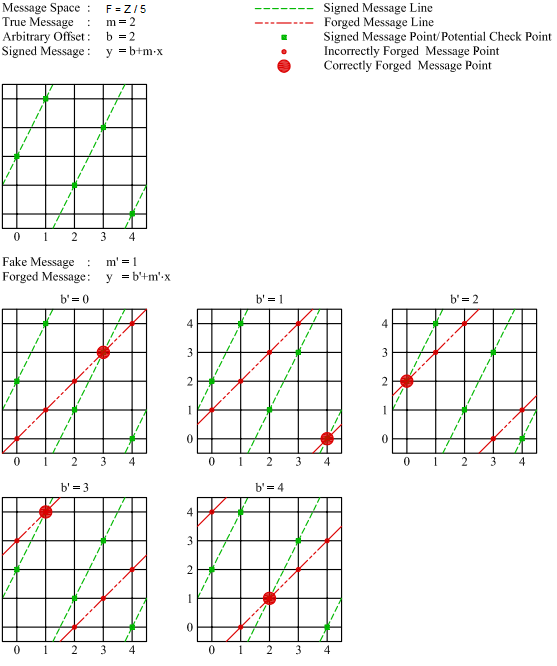
\includegraphics[width=\textwidth]{../../Graphics/PointAndLineExample.png}
\caption[Difficulty of forging a message]{Given a signed message ($m=2, b=2$) and a desired fake message ($m'=1$), each possible forged offset ($b'$) matches only one of the possible verifiers. Since the verifier is chosen at random, the chance of successful forging is $\frac{1}{|\mathbb{F}|}$.}
\label{img:ForgingVerifiableMessageForUnbounded}
\end{figure}

\subsection{Overview}

Like SBP, SUIP is based on a sequence of check rounds followed by a definitive round. SUIP's round messages are all specified in advance by the dealer. Each player has a list of messages to send, one per round. A message is composed of a $t$-of-$n$ share for the round secret, which is the true secret on the definitive round and random on other rounds, and accompanying $t$-of-$n$ shares for several round indicators, which are all 0 on the definitive round and random on other rounds. Players recognize the definitive round, and thus learn the secret is the round secret, by noticing when all of the round indicators are 0.

The dealer generates lists with distinct random lengths by starting from a minimum list length $\beta$, creating a list of that length with probability $\gamma$, called the marginal list termination probability, then repeating with the next highest length until $n$ list lengths have been chosen. Each list entry is a message with a round share, indicator shares, and verifiers and signatures to authenticate the shares. Each round the definitive round occurs with marginal termination probability $\alpha$, taking into account that after the shortest list has ended the definitive round must occur immediately.

The dealer gives a ``short message'' to all players that may contain a masked message based on how the protocol terminates. SUIP can terminate in two ways, based on the lengths of the lists of messages and the definitive round. Either the definitive round occurs before any of the players run out of messages to send, hereafter referred to as the ``normal case'', or it occurs on the round after a single player has run out of messages to send, hereafter referred to as the ``short case". The player who runs out of messages in the short case is called the ``short player''. The short message is the message that would have been sent by the short player, if they had not run out of messages, masked by adding its contents to the short player's previous message to ensure it can't be used when the short player is not participating.

All messages, except the short message (to prevent individual players from using it to detect the definitive round in the short case), are verified using the scheme explained in Section~\ref{sec:vermes}, to prevent message forging. Every player has verifiers for every message they expect to receive. Every player has signatures for every receiver for every message they expect to send. The short message is verified implicitly by the round indicators: when it is applied in the wrong round or to the wrong player it effectively randomizes the round indicators, meaning the probability they are all 0 can be made as small as necessary.

Each round every player broadcasts their message for the round to all other players and verifies the messages they receive. If there are at least $t$ available round messages then the round secret and round indicators are easily recovered and, if it is the definitive round, players will notice the round indicators are all $0$ and accept the correct secret. If there are fewer than $t-1$ available round messages then the round secret and round indicators can't be recovered and the protocol aborts. If there are exactly $t-1$ available round messages then the short case may be occurring and players attempt to use the short message to recover a $t$'th round message. For each player who did not send a valid message this round, but was cooperating until now, a potential round message is created by adding the short message's contents to the player's previous message's contents. If one of the potential short messages results in the round indicators all being 0 then the protocol succeeds. Otherwise the short case is not occurring and the protocol aborts.

See Algorithms \ref{alg:SUIP:Dealer} and \ref{alg:SUIP:Player} and Figure \ref{Ex:SUIP} for more details.

SUIP is derived from Kol and Noar's protocol for rational secret sharing~\cite{kol08} but is different in important respects. SUIP uses an authentication method that does not rely on computational difficulty, allows the definitive round to occur before the shortest list ends, and gives lists with distinct lengths to each player. Each of these differences has important security implications.

\begin{algorithm}
  \caption{Dealer Protocol for SUIP}
  \label{alg:SUIP:Dealer}
  \begin{algorithmic}
    \INPUT Finite field $\mathbb{F}$
    \INPUT Total number of shares $n$ and threshold $t$
    \INPUT Marginal probability of definitive round occurring $\alpha$
    \INPUT Minimum message list size $\beta$
    \INPUT Message list marginal termination probability $\gamma$ satisfying $\gamma \leq \alpha$
    \INPUT Secret value $s$ from $\mathbb{F}$
    \OUTPUT Ordered list of $n$ shares
    \STATE Choose the minimum number of indicators $\omega$ as explained in Section~\ref{Sec:SUIP:MinIndicators}
    \STATE Generate an ordered list $L$ of $n$ monotonically increasing list lengths
    	$$D_i = Random(Geometric(stopChance: \gamma))$$
    	$$L_1 = \beta + D_1 \text{, } \text{ } \text{ } L_i = L_{i-1} + 1 + D_i$$
    \STATE Uniformly shuffle the list lengths, noting the new index $c$ of the shortest list
    \STATE Choose the definitive round $r$ as explained in Section~\ref{Sec:SUIP:ChooseRound}
    \STATE Generate Shamir shares for the round secrets and indicators
    	$$S_{i} = CreateShamir(if(i = r, s, Random(\mathbb{F})), \mathbb{F}, n, t) \text{ for } i \in [1, max(L)+1]$$
    	$$I_{i,j} = CreateShamir(if(i = r, 0, Random(\mathbb{F})), \mathbb{F}, n, t) \text{ for } i \in [1, max(L)+1], j \in [1, \omega]$$
    \STATE Create signatures and verifiers for every secret share $S_i$ and indicate share $I_{i,j}$ for every pair of sending and receiving player
    \STATE Compute the short message $X$ composed of a masked secret share $X_0$ and masked indicator shares $X_{1..\omega}$
    	$$X_0 = S_{r,c} - S_{r-1,c} \text{, } \text{ } \text{ } X_j = I_{r,j,c} - I_{r-1,j,c} \text{ for } j \in [1, \omega]$$
    \STATE Return the ordered list $R$ of $n$ SUIP shares $R_i$
    	$$R_i = (i, X, S_{i,j}, I_{i,k,j}, VerifiersUpToRound(L_i+1), SignaturesUpToRound(L_i))$$
    	$$\text{for } i \in [1, n], j \in [1, L_i], k \in [1, \omega]$$
  \end{algorithmic}
\end{algorithm}

\begin{algorithm}
  \caption{Player Protocol for SUIP}
  \label{alg:SUIP:Player}
  \begin{algorithmic}
    \INPUT Finite field $\mathbb{F}$
    \INPUT Total number of shares $n$ and threshold $t$
    \INPUT Share index $i$
    \INPUT Upper bound $r_{ceil}$ on the number of rounds
    \INPUT List of $r_{ceil}-1$ signed secret shares $S$ and arrays of signed indicator shares $I$
    \INPUT List $V$ of $r_{ceil}$ verifiers for other players' secret shares and indicators
    \INPUT Short message $X$
    \OUTPUT Success with secret $s$ or failure
    \STATE Mark all players, identified by indexes in $[1, n]$, including ourselves, as cooperating
    \STATE Let $r = 1$
    \WHILE { true }
      \STATE If the number of cooperating players is less than $t$ then exit with failure
      \STATE If $r < r_{ceil}$ then broadcast our round message $S_r, I_r$ to all players, including ourselves
      \STATE Receive round messages, that match corresponding verifiers in $V_r$, from cooperators
      \STATE Mark any player who did not send a verified round message as non-cooperating
      \STATE Let $N$ be the set of non-cooperating players who were cooperating last round
      \STATE Let $n_{msg}$ be the number of verified round messages, counting ours if we sent one
      \STATE If $n_{msg} < t - 1$ then exit with failure
      \STATE Compute possible extra share sets, if necessary, by applying the short message to $N$
      		$$PossibleExtraSets = if(n_{msg} \geq t, \{\emptyset\}, \{\{LastMessage(e) + X\} | e \in N\}))$$
      \FOR {each $extra$ in $PossibleExtraSets$}
        \STATE Compute the round secret $s$ and indicators from verified and $extra$ shares
        \STATE If all round indicators are 0 then exit with secret $s$
      \ENDFOR
      \STATE Increment $r$ by $1$
    \ENDWHILE
  \end{algorithmic}
\end{algorithm}

\begin{figure}
  \caption{Example Dealer Run of SUIP}
  \label{Ex:SUIP}
  \begin{itemize}
    \item Finite Field $\mathbb{F}$ is the integers mod 5
    \item Share count is $n = 2$ and threshold is $t = 2$
    \item Marginal round termination probability is $\alpha = \frac{1}{2}$
    \item Minimum list size is $\beta = 1$ and marginal termination probability is $\gamma = \frac{1}{3}$
    \item Number of indicators is $\omega = 1$
    \item Secret is $s = 3$
    \item Generate list lengths $L_1 = 4, L_2 = 3$ and final round $r = 3$
    \item Generate $MaxLength+1$ Shamir shares for potential secrets and indicators
  
      \begin{tabular}{|r|r|r|r|r|}
      \hline
        Round & Potential Secret & Secret Shares & Indicator & Indicator Shares \\
      \hline
        1 & 2  & (1,2), (2,2) & 1 & (1,2), (2,3) \\
      \hline
        2 & 1  & (1,0), (2,4) & 1 & (1,1), (2,1) \\
      \hline
        3 & 3  & (1,4), (2,0) & 0 & (1,2), (2,4) \\
      \hline
        4 & 4  & (1,4), (2,4) & 4 & (1,3), (2,2) \\
      \hline
        5 & 3  & (1,3), (2,3) & 2 & (1,1), (2,0) \\
      \hline
      \end{tabular}
      
    \item Generate verification information for every sender/receiver/share triplet
    \subitem In round 1 the secret share for index 1 is 2, and there is only one receiver. An arbitrary line with slope 2 is 1+2x. An arbitrary point on that line is (1,3). So for this message, share 1 could include the line offset 1 and share 2 could include the check point (1,3).
    \subitem Verification information is omitted from this example for brevity.
    
    \item Trim shares' list of messages to the corresponding list lengths $L_1 = 4, L_2 = 3$
    \item Compute the short message (although it won't be used)
    \subitem $X_0 = 4 - 0 = 4$, $X_1 = 2 - 4 = 3$
    \subitem Will not be used because the definitive round occurs before it is needed
    \item Resulting shares (signatures/verifiers omitted for space)
    
      \begin{tabular}{|r|r|r|r|}
      \hline
        Index & Secret Shares & Indicator Shares & Signatures/Verifiers per receiver/sender \\
      \hline
        1 & 2, 0, 4, 4 & (2), (1), (2), (3) & \ldots, \ldots, \ldots, \ldots\\
      \hline
        2 & 2, 4, 0 & (3), (1), (4) & \ldots, \ldots, \ldots\\
      \hline
        short & 0 & (1) & -\\
      \hline
      \end{tabular}
  \end{itemize}
\end{figure}

\subsection{Analysis}

SUIP is relatively expensive to run, especially for the dealer, who has to simulate all player interactions. Let the finite field be $\mathbb{F}$, the number of players be $n$, the threshold be $t$, the marginal definitive round probability be $\alpha$, the marginal list termination probability be $\gamma$, the minimum list length be $\beta$, and number of indicators $\omega$. The expected number of rounds is $\frac{1}{\alpha}$. The expected size of the shortest list of messages is $\beta + \frac{1}{\gamma}$. The expected size of the longest list of messages is $\beta + \frac{n}{\gamma}$. The expected size of shares, dominated by the $O(n)$ verifiers and signatures needed for each entry in the longest list, is $O((\beta + \frac{n}{\gamma}) \times \omega \times n \times (log |\mathbb{F}|))$. The expected runtime of the dealer is $O((\beta + \frac{n}{\gamma}) \times n^2 \times (log |\mathbb{F}|) \times \omega \times Shamir(n, t))$. The expected runtime of the players is $O(\frac{1}{\alpha} \times n \times (log |\mathbb{F}|) \times \omega \times Shamir(n, t))$.

Because it is designed for potentially unbounded players, SUIP is expensive compared to its bounded variant SBP. SUIP's share sizes increase linearly with the expected number of rounds and indicators and quadratically with the number of players. By comparison, SBP's share sizes increase only with the number of players and only linearly in that respect. Additionally, unlike in SUIP, most of the information in SBP's shares is common to all the shares. The dealer costs in SUIP also scale poorly, because the dealer effectively simulates every player's interaction with every other player for every round, whereas in SBP the dealer can handle each player individually and can ignore non-definitive rounds.

Although SUIP is not immune to coalitions, it can be made arbitrarily close to immune to coalitions by adjusting the number of indicators $\omega$, marginal definitive round probability $\alpha$, minimum list length $\beta$, and marginal list termination probability $\gamma$. Given any desired probability $p$ of success satisfying $p < 1$, we can choose values for $\omega$, $\alpha$, $\beta$, and $\gamma$ that ensure running SUIP with at least $t$ rational players results in all rational players learning the secret with probability greater than $p$. Lemma~\ref{Lem:SUIP:RatNashCoop} shows that cooperating until the short case is a Nash equilibrium if $\alpha$ is small enough. Lemmas~\ref{Lem:SUIP:ShortPlayerCoalitionsPremptivelyKnowShortRound}, \ref{Lem:SUIP:MaxSizeCoalitionsPremptivelyKnowShortRound}, \ref{Lem:SUIP:MinimumThresholdAndShortCaseMeansNoOneLearnsSecret}, \ref{Lem:SUIP:ShortPlayerMayLearnSecretExclusively}, \ref{Lem:SUIP:AllCoalitionsTempted} and \ref{Lem:SUIP:MaxSizeCoalitionsTemptedMore} cover the various ways the short case allows players to misbehave and Lemmas~\ref{Lem:SUIP:NoPlayerLearningSecretIsReducible}, \ref{Lem:SUIP:ShortPlayerLearningSecretExclusivelyIsReducible}, and \ref{Lem:SUIP:HighTemptationAvoidable} show adjusting $\beta$ and $\gamma$ makes these problems sufficiently unlikely. Finally, Lemma~\ref{Lem:SUIP:MaliciousImmune} proves SUIP is immune to malicious coalitions if $\omega$ is large enough.

\begin{lemma}\label{Lem:SUIP:RatNashCoop}Given a small enough $\alpha$, cooperating until the short round is a Nash equilibrium for rational players and rational coalitions.\end{lemma}

Before the short round rational players and coalitions experience a temptation of at most $\alpha$, because they don't have the $t$ shares necessary to determine if the following round is the definitive round or not. Therefore, before the short round, cooperating is a Nash equilibrium for the same reasons outlined in the equivalent lemma for SBP, Lemma~\ref{Lem:SBPRatNash}: the expected payoff for defecting can be made arbitrarily small by decreasing $\alpha$.

\begin{lemma}\label{Lem:SUIP:ChanceOfShortCase}The short case occurs with probability $(1-\alpha)^\beta \times \frac{\gamma}{\alpha}$.\end{lemma}
\begin{proof}
In order to reach the short case the protocol must have enough rounds to exceed the minimum list length. This occurs with probability $(1-\alpha)^\beta$. After the minimum list length is exceeded the probability of the definitive round being a short case is its marginal probability over the marginal probability of the definitive round, which is $\frac{\gamma}{\alpha}$. The probability of the short case occurring is their product.
\end{proof}

\begin{lemma}\label{Lem:SUIP:ShortPlayerCoalitionsPremptivelyKnowShortRound}In the short case, coalitions containing the short player can detect the definitive round before it starts.\end{lemma}
\begin{proof}
If a player has no messages to send in the coming round then they know that the short case is occurring, that they are the short player, and that the coming round must be the definitive round. Therefore when a coalition has a player with no more messages to send, who must be the short player, they know the next round must be the definitive round before it starts.
\end{proof}

\begin{lemma}\label{Lem:SUIP:MaxSizeCoalitionsPremptivelyKnowShortRound}When the short player is present and the short case occurs, all coalitions of size $t-1$, or individual players when $t = 2$, can detect the definitive round before it starts.\end{lemma}
\begin{proof}
Let $C$ be a set of $t-1$ colluding players. Let $d$ be the short player. Let $r$ be the definitive round, occurring after $d$'s list of messages is exhausted.

Either $d \in C$ or $d \notin C$.

If $d \in C$ then the colluding players can detect the definitive round before it starts by Lemma~\ref{Lem:SUIP:ShortPlayerCoalitionsPremptivelyKnowShortRound}.

If $d \notin C$ then, after round $r-1$, the members of $C$ have enough round messages to determine if the short message will apply to any of the players outside of $C$ by simulating the next round as if all other players sent no messages. When the short player $d$ is present in the round before the definitive round in the short case they will be able to simulate applying the short message to $d$, see that the resulting round indicators are all $0$, learning the secret and that the next round is the definitive round before it starts.

A coalition of $t-1$ colluding players, or an individual player when $t=2$, can pre-emptively detect the definitive round whether or not they include the short player, as long as the short player is present and the short case occurs.
\end{proof}
 
\begin{lemma}\label{Lem:SUIP:MinimumThresholdAndShortCaseMeansNoOneLearnsSecret}When $t=2$ and the short case occurs, no one learns the secret.\end{lemma}
\begin{proof}
When $t=2$ all players will pre-emptively detect the definitive round in the short case, by Lemma~\ref{Lem:SUIP:MaxSizeCoalitionsPremptivelyKnowShortRound}, and will want to defect.

All players who are not the short player will be able to defect on the definitive round. The short player is unable to defect on the definitive round, because the protocol doesn't place any constraints on their actions. But, because the short player knows all other players will defect on the round after the short player's list runs out, the short player has no incentive to cooperate on the preceding round. Thus the short player will defect one round before the short case's definitive round.

Thus all players defect before or during the definitive round, meaning no definitive round messages are broadcast and therefore no player learns the secret.
\end{proof}

\begin{lemma}\label{Lem:SUIP:NoPlayerLearningSecretIsReducible}By choosing a large enough $\beta$, the probability of all players not learning the secret due to Lemma~\ref{Lem:SUIP:MinimumThresholdAndShortCaseMeansNoOneLearnsSecret} can be made arbitrarily small.\end{lemma} 
\begin{proof}
As explained in Lemma~\ref{Lem:SUIP:MinimumThresholdAndShortCaseMeansNoOneLearnsSecret}, no player will learn the secret in the short case when $t=2$. But by Lemma~\ref{Lem:SUIP:ChanceOfShortCase} the short case has probability that decreases exponentially as $\beta$ increases. We can make the probability of all players not learning the secret arbitrarily small by increasing $\beta$.
\end{proof}

\begin{lemma}\label{Lem:SUIP:ShortPlayerMayLearnSecretExclusively}When $t=2$, the short player can learn the secret exclusively if the definitive round is the last round for which the short player has a message.\end{lemma} 
\begin{proof}
As explained in the proof of Lemma~\ref{Lem:SUIP:MinimumThresholdAndShortCaseMeansNoOneLearnsSecret}, the short player will defect one round before the definitive round would occur due to the short case when $t=2$. When this round happens to be the definitive round in the normal case and there are exactly 2 remaining rational players, one of which is the short player, the short player will unilaterally defect and learn the secret exclusively.
\end{proof}

\begin{lemma}\label{Lem:SUIP:ShortPlayerLearningSecretExclusivelyIsReducible}By choosing a large enough $\beta$, the probability of the short player learning the secret exclusively due to Lemma~\ref{Lem:SUIP:ShortPlayerMayLearnSecretExclusively} can be made arbitrarily small.\end{lemma} 
\begin{proof}
As explained in the proof of Lemma~\ref{Lem:SUIP:MinimumThresholdAndShortCaseMeansNoOneLearnsSecret}, the short player will defect on the round before they know the short case would occur due to their list running out. As explained in the proof of Lemma~\ref{Lem:SUIP:ShortPlayerMayLearnSecretExclusively}, in order for the short player to learn the secret exclusively, the round they defect on must be the definitive round due to the normal case. The probability of that occurring is the probability that the protocol ends in the normal case but would have ended in the short case if there had been another round.

If the shortest list has the minimum length $\beta$ then the probability of the definitive round being the round before the short case would have occurred is $(1-\alpha)^{\beta-1} \times \alpha \times \gamma$. If the shortest list does not have the minimum length then the probability is $(1-\alpha)^\beta \times (1 - \frac{\gamma}{\alpha}) \times \gamma$. Together they give an upper bound on the probability of the short player exclusively learning the secret:

$$\gamma \times (1-\alpha)^{\beta-1} \times (\alpha + (1-\alpha) \times (1 - \frac{\gamma}{\alpha}))$$

Since this upper bound decreases exponentially as $\beta$ increases, we can make the probability of the short player exclusively learning the secret arbitrarily small by increasing $\beta$.
\end{proof}

\begin{lemma}\label{Lem:SUIP:NonColludersNotTemptedExceptT2}When $t > 2$, for non-colluding rational players, SUIP has constant temptation $\alpha$.\end{lemma}
\begin{proof}
The definitive round is chosen in a way that ensures each round has a marginal probability $\alpha$ of being the definitive round, as explained in Section~\ref{Sec:SUIP:ChooseRound}. Individual rational players do not have enough indicator shares to determine if a round is the definitive round in the normal case until it has finished. If they are not the short player then they can't detect the definitive round in the short case, because they still believe they are in the normal case and can't simulate applying the short message because $t > 2$. If they are the short player then by the time they can detect the definitive round they are unable to defect, because the short player's actions or lack thereof during the definitive round have no effect on the protocol's outcome.

Therefore, when $t > 2$, non-colluding rational players either can't defect or believe they will learn the secret with probability $\alpha$ if they defect.
\end{proof}

\begin{lemma}\label{Lem:SUIP:AllCoalitionsTempted}For rational coalitions $C$ up to size $t-2$ when $t \geq 4$, or individual players when $t=3$, SUIP has worst deal maximum temptation $1$ and expected deal maximum temptation $\alpha + (1-\alpha)^{\beta+1} \times \frac{\gamma}{\alpha} \times \frac{|C|}{n}$.\end{lemma}
\begin{proof}
If a coalition contains the short player and the short case occurs then, by Lemma~\ref{Lem:SUIP:ShortPlayerCoalitionsPremptivelyKnowShortRound}, they will pre-emptively detect the definitive round. This will allow them to defect without decreasing their chances of learning the secret. They encounter a temptation of $1$. If the short player is outside the coalition or the normal case occurs, then the coalition experiences a constant temptation of $\alpha$.

The dealer assigns the short message to a random player when generating the shares. The probability of a coalition $C$ containing the short player is $\frac{|C|}{n}$. The probability of the short case is, by Lemma~\ref{Lem:SUIP:ChanceOfShortCase}, $p_{short} = (1-\alpha)^\beta \times \frac{\gamma}{\alpha}$. The worst deal maximum temptation, based on the short case occurring and the short player being in the coalition, is $1$. The expected deal maximum temptation is $1 \times p_{short} \times \frac{|C|}{n} + \alpha \times (1 - p_{short} \times \frac{|C|}{n})$, which expands and re-arranges to $\alpha + (1-\alpha)^{\beta+1} \times \frac{\gamma}{\alpha} \times \frac{|C|}{n}$.
\end{proof}

\begin{lemma}\label{Lem:SUIP:MaxSizeCoalitionsTemptedMore}For rational coalitions of size $t-1$, and individual players when $t=2$, SUIP has worst deal maximum temptation $1$ and expected deal maximum temptation $\alpha + (1-\alpha)^{\beta+1} \times \frac{\gamma}{\alpha}$.\end{lemma}
\begin{proof}
By Lemma~\ref{Lem:SUIP:MaxSizeCoalitionsPremptivelyKnowShortRound}, coalitions of size $t-1$ can pre-emptively detect the definitive round in the short case. In that case they can defect and still be guaranteed to learn the secret. The short case is a possible deal, so the worst deal maximum temptation is $1$. By Lemma~\ref{Lem:SUIP:ChanceOfShortCase} the probability of the short case is $p_{short} = (1-\alpha)^\beta \times \frac{\gamma}{\alpha}$.

A deal that causes the short case has a maximum temptation of $1$ for the coalition. Otherwise the coalition experiences a constant temptation of $\alpha$. The expected maximum temptation of a deal is the maximum temptation of both cases weighted by their likelihood, which is $1 \times p_{short} + \alpha \times (1-p_{short})$ which expands and re-arranges into $\alpha + (1-\alpha)^{\beta+1} \times \frac{\gamma}{\alpha}$.
\end{proof}

\begin{lemma}\label{Lem:SUIP:HighTemptationAvoidable}By choosing a large enough $\beta$, the probability of a deal of SUIP having maximum temptation $\alpha$ can be made arbitrarily high.\end{lemma}
\begin{proof}
The cases where rational players or coalitions can pre-emptively detect SUIP's definitive round, explained in Lemmas~\ref{Lem:SUIP:ShortPlayerCoalitionsPremptivelyKnowShortRound} and \ref{Lem:SUIP:MaxSizeCoalitionsPremptivelyKnowShortRound}, are contained to the short case. In the normal case players always believe the next round is the definitive round with probability at most $\alpha$.

By Lemma~\ref{Lem:SUIP:ChanceOfShortCase}, the probability of the short case occurring is $(1-\alpha)^\beta \times \frac{\gamma}{\alpha}$. Since this probability decreases exponentially as $\beta$ increases, we can make the probability of the short case arbitrarily small. Therefore we can make the probability of a deal of SUIP having maximum temptation $\alpha$ arbitrarily high by increasing $\beta$.
\end{proof}

\begin{lemma}\label{Lem:SUIP:MaliciousImmune}By choosing a large enough $\omega$, SUIP is immune to malicious coalitions.\end{lemma}
\begin{proof}
During a round a player can either send the right message, a fake message, or no message. Sending no message or a fake message corresponds to defecting. Malicious players will defect before or during the definitive round, because otherwise the other players will have more definitive round shares and will be more likely to learn the secret.

If a player sends no round message then they are marked as non-cooperating by all cooperating players (see Algorithm \ref{alg:SUIP:Player}). If a player sends a fake message then the message verification step detects the forgery with arbitrarily high probability, and the player is marked as non-cooperating by all cooperating players. Coalitions have multiple chances to send a fake message, but the probability of all the fake messages being detected is still arbitrarily high based on the verification scheme.

A player who has been marked non-cooperating by all cooperating players is effectively absent from the protocol after the current round finishes. The other players attempt to apply the short message to the defector then ignore them in future rounds. The defector is sent no messages and the messages they send are discarded. The protocol will terminate as if it had started without the non-cooperating players being present because the outcome of a round doesn't depend on information from players who did not cooperate in previous rounds.

The probability of the short message being misapplied to a defecting player can be made arbitrarily low by choosing a large enough $\omega$ as explained in Section~\ref{Sec:SUIP:MinIndicators}. Therefore defectors are detected with arbitrarily high probability and applying the short message to them will not result in players learning the wrong secret with arbitrarily high probability. Therefore malicious players' effect on the protocol is equivalent to the effect of absent players.
\end{proof}

\subsection{Choosing a definitive round with the proper distribution}
\label{Sec:SUIP:ChooseRound}

Every round must have a marginal probability $\alpha$ of being the definitive round. But once we exceed round $\beta$ there are two ways to terminate: the normal way and due to the shortest list ending. The shortest list has a marginal probability $\gamma$ of terminating and we want an overall marginal probability $\alpha$ of termination. The marginal termination probability $x$ for the normal case should satisfy $\gamma + x \times (1 - \gamma) = \alpha$. Solving for $x$ gives $x = \frac{\alpha - \gamma}{1 - \gamma}$.

Algorithm \ref{alg:SUIP:DefinitiveRound} details how to choose a definitive round $r$ with an overall geometric distribution, given that we have already generated a random shortest list length $L_c = \beta + RandomGeometric(\gamma)$ and we must satisfy $r < L_c$.

\begin{algorithm}
  \caption{Choosing SUIP's Definitive Round}
  \label{alg:SUIP:DefinitiveRound}
  \begin{algorithmic}
    \INPUT The marginal definitive round probability $\alpha$ 
    \INPUT The minimum possible list length $\beta$
    \INPUT The marginal end of list probability $\gamma$ satisfying $\gamma < \alpha$
    \INPUT Length $L_c$ of the shortest list of messages
    \OUTPUT The definitive round $r$
    \STATE Let $r = 1$
    \WHILE { $r \leq \beta$ }
      \STATE Let $b$ be true with probability $\alpha$
      \STATE If $b$ is true then Return $r$
      \STATE Increment $r$ by 1 
    \ENDWHILE
    \WHILE { $r \leq L_c$ }
      \STATE Let $b$ be true with probability $\frac{\alpha - \gamma}{1 - \gamma}$
      \STATE If $b$ is true then Return $r$
      \STATE Increment $r$ by 1
    \ENDWHILE
    \STATE Return $r$
  \end{algorithmic}
\end{algorithm}

\subsection{Choosing a Large Enough Number of Indicators $\omega$ to Prevent Malicious Use of the Short Message}
\label{Sec:SUIP:MinIndicators}

When the short message is applied to the wrong player or in the wrong round, the resulting indicators are effectively random. If they happen to all be 0 then players will accept the wrong secret instead of aborting the protocol. Because malicious coalitions of unbounded players can compute these cases, we need to bound the probability of any such ``bad" cases existing.

Suppose our goal is to ensure the probability of a bad case existing is less than $\frac{1}{p}$ for some value $p$. There is a $\frac{1}{|\mathbb{F}|^\omega}$ chance of $\omega$ indicators randomly coming up 0. If there are $r$ rounds, $n$ players, and the threshold is $t$ then there are $\binom{n}{t} \times t \times r$ ways the short message can be applied. The probability of a bad case existing is thus $\frac{\binom{n}{t} \times t \times r}{|\mathbb{F}|^\omega}$. Solving $\frac{\binom{n}{t} \times t \times r}{|\mathbb{F}|^\omega} < \frac{1}{p}$ for $\omega$ gives $\omega > log_{|\mathbb{F}|} (\binom{n}{t} \times t \times r \times p)$.

Our bound for $\omega$ depends on the number of rounds $r$, but this is not ideal since it may ``leak" information about $r$ to the players via $\omega$. Since $r$ is a random variable, we can spend some of our probability bound choosing a high enough cut-off value $r'$. If we choose to allocate a $\frac{1}{2 p}$ probability to not exceeding the cut-off and the remaining $\frac{1}{2 p}$ probability to ensuring there are no bad cases when we don't exceed the cut-off, then we meet the overall bound of $\frac{1}{p}$. We solve for the cut-off round $r'$ using the fact that $r$ follows a geometric distribution parameterized by $\alpha$: $(1 - \alpha)^{r'-1} \leq \frac{1}{2 p}$, which solves to $r' \geq 1 + log_{\frac{1}{1-\alpha}}(2 p)$. We get our final bound by updating our previous $r$-dependent bound, feeding in a maximum probability of $\frac{1}{2 p}$ and the minimum value of $r'$:

$$\omega > \left(log_{|\mathbb{F}|} (2 p)\right) + \left(log_{|\mathbb{F}|} \left(1 + log_{\frac{1}{1-\alpha}}(2 p)\right)\right) + log_{|\mathbb{F}|} \left(\binom{n}{t} \times t\right)$$

For practical cases ($|F| \geq 2^{256}, n \leq 200, \alpha \geq \frac{1}{100}, p \leq 2^{256}$) a large enough value of $\omega$ is 2. For theoretical cases, the minimum number of indicators grows logarithmically against the magnitude or inverse magnitude of the protocol's parameters and $p$. Therefore we can practically achieve an arbitrarily high probability of the short message not being abusable.

\subsection{Observation and Conjecture about the Short Case's Consequences and Necessity}

The primary complicating factor in running and analyzing SUIP is the existence of the short case. In particular, it is the reason the protocol must have some probability of failing in the presence of rational players who want to cooperate until they learn the secret. A protocol with a short case can't be immune to rational coalitions, although it can be arbitrarily close.

The short case has particularly high costs for the $t=n=2$ case. Every 2-of-2 protocol with a short case must choose between everyone learning the secret in the short case or not learning the wrong secret when the other player is malicious. SUIP prevents a malicious player from convincing the other player to accept the wrong secret. Kohl and Noar's 2-of-2 protocol~\cite{kol08} guarantees two rational players will both learn the secret. The trade-off is a consequence of deciding whether or not, when a player appears to defect, the remaining player can check if the short case is occurring. If the remaining player can check for the short case then they can do so before the definitive round starts, learn the secret, stop participating, and thus prevent the short player from learning the secret. If the remaining player can't check for the short case then they can't distinguish between the short case occurring and a malicious player defecting on a non-definitive round.

Any protocol based on a non-interacting dealer giving players lists of messages to send will have an equivalent to the short case. This is a consequence of the players using the length of the lists to derive a maximum value for the definitive round. The protocol must sometimes last until a round where a player knows it is the definitive round and then that player will want to defect. When that occurs, the protocol is ending in a short case.

Removing the short case from a protocol is not trivial. For example, if you attempt to eliminate the short case by having the dealer recreate shares until the short case does not occur, players can use that knowledge to get better bounds on the maximum value of the definitive round and a new type of short case is created as a result.

Players need an unbounded amount of entropy when opponents may be unbounded, because otherwise players will sometimes deduce each other's state and break the security of the protocol, and that entropy must either come from the dealer or the players. It is convenient, and perhaps necessary, for the entropy to come from the dealer in order to allow for verification. But when the entropy comes from the dealer the protocol must have a short case. Whether or not entropy generated by the players can be properly verified is an avenue for future work.


\subsection{Summary}

SUIP is derived from Kol and Noar's protocol for rational secret sharing~\cite{kol08} and improves upon it primarily by making the short case an exceptional case instead of the required case. SUIP's security is derived from missing information, not computational difficulty, meaning players with unbounded computational capacity have no advantage over ``normal" players. SUIP is immune to malicious coalitions and, except for vulnerabilities caused by the short case, is immune to rational coalitions. When the short case occurs, and there are coalitions or $t=2$, some players may not learn the secret.

We anticipate future work related to SUIP to focus on eliminating the short case or reducing its effects. If the short case can't be eliminated then we conjecture that no protocol for unbounded players achieves immunity against rational coalitions. We also expect techniques from SUIP to be applicable to asynchronous protocols for unbounded players, a case which this thesis does not explore.





\chapter{Asynchronous Broadcast}
\label{chapter:Asynchronous}

In practice, communication is not synchronous. The internet, for example, is based on asynchronous messages. Protocols that assume synchronous broadcast can't be naively deployed over the internet without breaking their basic assumptions and compromising their security.

Asynchronous broadcast is like synchronous broadcast, except it does not allow for senders to synchronize their sends. As a consequence, rational players, who have an incentive to wait to receive messages before sending their messages, will tend to deadlock waiting for their rational peers unless the protocol specifies a message ordering. Asynchronous broadcast still assumes reliability, timeliness, and consistency across receivers. If a sender chooses to send a message then all receivers will receive the same message in bounded time. If a sender chooses to send no message, then all receivers will know, in bounded time, no message was sent.

This chapter presents consequences of using asynchronous broadcast instead of synchronous broadcast for rational secret sharing. It also presents two asynchronous protocols: one for conspicuous secrets and one for inconspicuous secrets.

\section{Limitations of all Asynchronous Rational Secret Sharing Protocols}
\label{Sec:AsympWeak}

Asynchronous protocols are more restricted than synchronous protocols, but it is not immediately obvious whether or not they are necessarily weaker as a consequence. This section proves that asynchronous protocols are weaker, particularly if the secret is conspicuous.

As shown in Lemma~\ref{Lem:Async:ConspicuousMustSacrifice}, asynchronous protocols for conspicuous secrets must ``sacrifice'' at least one player. It is impossible for a protocol to guarantee all rational players will learn the secret, because the last sender would know the secret and have no incentive to send. Inconspicuous protocols can avoid this problem because they allow for the last sender to have the secret but not know it is the secret until other players refuse to send messages in response.

Lemma~\ref{Lem:Async:CoalitionsMayPreempt} proves asynchronous protocols are vulnerable to coalitions ``pre-emptively" learning the secret, by pre-sharing messages internally, meaning they learn the secret earlier than any player could have without collusion. Pre-emptively learning the secret allows a coalition to defect earlier, potentially depriving other players of shares and causing them to not learn the secret. As shown in the proof, every coalition $C$ has at least a $\frac{|C| \times (|C| - 1)}{n \times (n-1)}$ probability of pre-emptively learning the secret. This lower bound can probably be strengthened, because it is derived using simplifying assumptions.

Finally, we prove in Lemma~\ref{Lem:Async:NoConspGoodRatImmune} that no conspicuous asynchronous protocol is immune to rational coalitions if more than a strict majority of the players can learn the secret because of coalitions' ability to pre-emptively learn the secret. This proof does not extend trivially to inconspicuous asynchronous protocols. An inconspicuous protocol can ensure that, by the time a coalition can learn the secret, all players have the secret value but do not yet \emph{know} that they have the secret value. A protocol where players fall back to accepting their current potential secret when the protocol ``fails" can be immune to rational coalitions. However, this fall-back strategy can be abused by malicious coalitions to cause players to accept an incorrect potential secret. We conjecture a weaker property for inconspicuous asynchronous protocols: every asynchronous protocol either doesn't allow a strict majority of the players to learn the secret, is not immune to malicious coalitions, or is not immune to rational coalitions.


\begin{lemma}\label{Lem:Async:ConspicuousMustSacrifice}If all players are rational, the secret is conspicuous, and communication is asynchronous then at least one player will not learn the secret.\end{lemma}
\begin{proof}
We will prove this result by contradiction. Assume all players learn the secret.

The protocol is divided into rounds with a single sender per round, by definition from Section~\ref{Def:Broadcast}. Let $r$ be the first round such that, at the end of round $r$, all players are guaranteed to eventually know the secret even if the others stop cooperating. Let $s$ be the expected sender of round $r$'s message.

Because the secret is conspicuous, players know whether or not they have the secret. Therefore a player can simulate the other players defecting in order to learn the secret as soon as they are guaranteed to eventually know the secret. A player can't have a conspicuous secret and not know it. The sender $s$ either has the secret before round $r$ and knows about having it or doesn't have the secret before round $r$ and knows about not having it.

If $s$ doesn't have the secret before round $r$ then, because $s$ received no information during round $r$ because $s$ was the sole sender, $s$ still does not know the secret after round $r$. But all players know the secret after round $r$, so $s$ must have known the secret before round $r$.

If $s$ knows the secret before round $r$ then $s$ has no incentive to send a correct message during round $r$. The sender $s$ would know the secret and know sending a correct message could only help the other players learn the secret which, because $s$ is rational, $s$ wants to prevent from happening. Therefore $s$ will not send a correct message in round $r$ when they know the secret.

Since $s$ must have known the secret before round $r$ they would have not sent a correct message. Therefore no players receive new information during round $r$, meaning no players can learn the secret due to round $r$, contradicting the definition of $r$. Contradiction.

The assumption that all players learn the secret creates a contradiction.

At least one player did not learn the secret.
\end{proof}

\begin{lemma}\label{Lem:Async:CoalitionsMayPreempt}If all players are rational and communication is asynchronous then there is a probability bounded away from 0 of a coalition of randomly chosen players learning the secret before any individual player could.\end{lemma}
\begin{proof}
The protocol is divided into rounds with a single sender per round, by definition from Section~\ref{Def:Broadcast}. 
Let $n$ be the number of players.
Let $C$ be a rational coalition of players, selected randomly, with size less than the threshold $t$.
Let $r$ be the first round where a player would have learned the secret if there were no collusion.
Let $L$ be the set of learners: players who learn the secret in round $r$.
Let $s$ be the sender of round $r$'s message.
The sender cannot be one of the learners because the sender is receiving no new information during round $r$.

If the sender and at least one of the learners are in the coalition, then the coalition can internally simulate sending round $r$'s message before round $r$ occurs and thereby pre-emptively learn the secret. The probability of this occurring is $\frac{|C|}{n} \times \left(1 - \frac{\binom{n - |C|}{|L|}}{\binom{n - 1}{|L|}}\right)$. This function varies with $L$, which the protocol has some control over. Higher values of $L$ give higher probabilities, so a lower bound for any protocol is setting $L$ to its minimum value: 1. This gives a lower bound probability of $\frac{|C| \times (|C| - 1)}{n \times (n-1)}$, which is independent of the protocol.
\end{proof}

\begin{lemma}\label{Lem:Async:NoConspGoodRatImmune}There is no asynchronous protocol for conspicuous secrets that both guarantees more than $\lceil \frac{n}{2} \rceil$ of the players learn the secret and is immune to all rational coalitions.\end{lemma}
\begin{proof}
The protocol is divided into rounds with a single sender per round, by definition from Section~\ref{Def:Broadcast}. Before a round $r$ a player $p$ has some minimum number $m(p, r)$ of other players that must continue cooperating in order for $p$ to learn the secret. If $p$ learns the secret when round $r$ finishes then $m(p, r) = 1$, because $p$ must have received a message from the round's sender that allowed $p$ to learn the secret, and $m(p, r+1) = 0$. The number of cooperating players a given player needs can decrease by either 0 or 1 each round, so we can further derive that $m(p, r-i) \leq 1+i$.

Let $h(r)$ be the minimum value of $m(p, r)$ for any player on round $r$. If at least one player learns the secret, and the protocol satisfies the basic correctness requirement that $t$ players are needed in order for any to learn the secret, then for any $i \in [0, t]$ there will be a round where $h(r) = i$.

Suppose a rational coalition $C$ has size $|C|$ satisfying $1 < |C| < t$. Let $r_0$ be the smallest round such that $h(r) = |C|-1$. In round $r_0$ there is a player who depends on at most $|C|-1$ other players. If that player is in the coalition, and the potential dependees are the other players in the coalition, then the coalition can learn the secret and defect. This leaves at most $n-|C|$ cooperating players, all of whom need at least $|C|-1$ other players to be present in order to learn the secret due to how we choose $r_0$. If $n < 2 |C|$ then they can't learn the secret and will fail.

When the number of players who would have learned the secret if the protocol had been run without the coalition is larger than $\lceil \frac{n}{2} \rceil$, they can't all be placed in the coalition. This ensures that the coalition defecting on round $r$ causes fewer players to learn the secret than if the coalition had not been present. Therefore the protocol is not immune to all rational coalitions, because the presence of a rational coalition can cause fewer players to learn the secret.
\end{proof}

 




\section{Asynchronous Protocol for Conspicuous Secrets and Bounded Opponents}
\label{Sec:ABCP}

Asynchronous protocols require trade-offs that synchronous protocols don't have to make. For example, as shown in Lemma~\ref{Lem:Async:ConspicuousMustSacrifice}, an asynchronous protocol that works for conspicuous secrets must ``sacrifice'' at least one player (if all players are rational then one will not learn the secret). It is also impossible to guarantee more than a strict majority of players learn the secret while maintaining immunity against rational coalitions, as shown in Lemma~\ref{Lem:Async:NoConspGoodRatImmune}.

The protocol presented in this section, named ABCP (asynchronous bounded conspicuous protocol), is an asynchronous protocol for conspicuous secrets (and bounded opponents). It guarantees that at most $t-1$ non-colluding rational players are sacrificed, but allows for only $1$ player to be sacrificed if all players are non-colluding and rational.

\subsection{Overview}

ABCP is like SBP except the definitive round is ``spread out'', meaning different players learn the secret after different rounds. This allows players who send later to be incentivized into participating for one more round by delaying when they learn the secret.
 
ABCP is based on a sequence of check rounds followed by a block of $n$ definitive rounds during which a player learns shares of the true secret. Players take turns sending messages in a round robin format. The start of the block of definitive rounds is different for each player and chosen so that, when they are supposed to send their last message, they will need a specified number of additional shares before they learn the secret. Each round every player sends a message created by a verifiable random function (VRF). Each player takes received messages and offsets them to create round shares. The offset applied is different for each ordered pair of sender and receiver, but does not depend on the round. Both the offsets and VRFs are chosen beforehand by a dealer.

Before a player's definitive block of rounds the round shares they compute are random. The offsets and VRFs are chosen by the dealer to ensure that during the player's definitive block of rounds the round shares they compute are the Y coordinates of Shamir shares for the secret with a threshold of $t$. Players recognize the definitive round by combining the round shares and matching the result against a bit commitment to the secret provided by the dealer. Each player's definitive block of rounds is positioned so that the earliest round they can learn the secret is a specified number $\delta$, called the ``share shortage", of rounds after a round where they send a message.

See Algorithms \ref{alg:ABCP:Dealer} and \ref{alg:ABCP:Player} and Figure \ref{img:ex:ABCP} for details.

\begin{algorithm}
  \caption{Dealer Protocol for ABCP}
  \label{alg:ABCP:Dealer}
  \begin{algorithmic}
    \INPUT Finite field $\mathbb{F}$, number of shares $n$, and threshold $t$
    \INPUT Share shortage $\delta$ satisfying $0 < \delta < t$
    \INPUT Marginal probability of termination $\alpha$
    \INPUT Verifiable random function scheme $VRFS$ and commitment scheme $CS$
    \INPUT Secret value $s$ from the finite field $\mathbb{F}$
    \OUTPUT An ordered list of $n$ ABCP shares for the secret $s$ with a threshold of $t$
    \STATE Create a commitment $c$ to the secret $s$
    	$$c = CS.CreateCommitment(s)$$
    \STATE Create ordered lists $V$ and $G$ of $n$ public ($V$) and private ($G$) VRFS key pairs
    	$$V_i, G_i = VRFS.NewKeyPair()$$
    \STATE Pick the earliest definitive round of any share $b$ 
	    $$b = Random(UniformDistribution([0,n))) + Random(Geometric(\alpha))$$
    \STATE Compute the starting round $r_i$ satisfying $r_i \geq b$ of each share's block of definitive rounds based on the desired share shortage by also satisfying $r_i + t - 1 - \delta = i \pmod{n}$
  	    $$r_i = b + ((i-b-t+\delta+1) \text{ } mod \text{ } n)$$
    \STATE Create $n$ ordered lists $S_i$ of $n$ Shamir shares (points) $S_{i,j}$ with threshold $t$ for the secret
  	    $$S_i = CreateShamirShares(s, \mathbb{F}, n, t) \text{ } for \text{ } i \in [1, n]$$
  	    $$XOfPoint(S_{i,j}) = j \text{ } for \text{ } i,j \in [1, n]$$
    \STATE Compute the $n$ ordered lists $Y_i$ of $n$ offsets $Y_{i,j}$
  	    $$Y_{i,j} = VRFS.ValueOf(G_j, r_i + (j-r_i \pmod{n})) + S_{i,j}$$
    \STATE Return the list $R$ of $n$ ABCP shares composed of the commitment, all public keys, share-specific offsets, an index, and a private key
    	$$R_i = (c, V, Y_i, i, G_i)$$
  \end{algorithmic}
\end{algorithm}
\begin{algorithm}
  \caption{Player Protocol for ABCP}
  \label{alg:ABCP:Player}
  \begin{algorithmic}
    \INPUT Finite field $\mathbb{F}$
    \INPUT Total number of shares $n$ and threshold $t$
    \INPUT Verifiable random function scheme $VRFS$ and commitment scheme $CS$
    \INPUT Share index $i \in [1, n]$
    \INPUT VRFS private key $G_i$
    \INPUT Ordered list $V$ of $n$ VRFS public keys
    \INPUT Ordered list $Y_i$ of $n$ offsets
    \INPUT Secret commitment $c$
    \OUTPUT Secret value or failure
    \STATE Mark all players, identified by indexes in $[1,n]$, including ourselves, as cooperating
    \STATE Let $Q$ be an empty queue of points in $\mathbb{F}^2$
    \STATE Let $r = 1$
    \WHILE {true}
	  \STATE If fewer than $t$ players are marked as cooperating then exit with failure
	  \STATE Let $x$ be the player with index $j$ satisfying $j \equiv r \pmod{n}$
	  \IF {$j = i$} 
	  	 \STATE Broadcast the message $VRFS.ValueAndProof(G_i, r)$ to all cooperating players
	  \ENDIF
	  \STATE Let $m, w$ be the message value and proof received from $x$ (if any) in round $r$
	  \STATE If $x$ sent no message or a message failing $VRFS.Verify(V_j, m, w)$ then mark $x$ as non-cooperating
	  \STATE If $x$ is marked as non-cooperating then skip to the next round
	  \STATE Enqueue the point $(j, m + Y_{i,j})$ into $Q$
      \STATE If $Q$ has more than $t$ items then dequeue the oldest item from $Q$
	  \IF {$Q$ has $t$ items}
	   	\STATE Let $P$ be the polynomial interpolated from the points in $Q$
	    \STATE If $CS.Matches(c, P(0))$ then exit with the secret $P(0)$
	  \ENDIF
      \STATE Increment $r$ by $1$
	\ENDWHILE
  \end{algorithmic}
\end{algorithm}
\begin{figure}
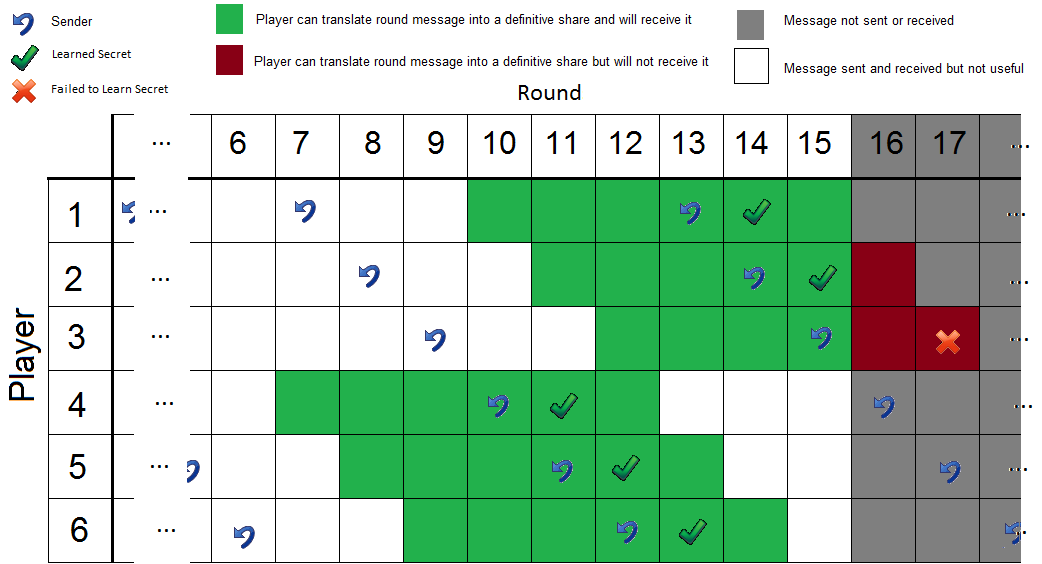
\includegraphics[width=\textwidth]{../../Graphics/AsyncVerifiedSecret_n6t5d1.png}
\caption[Shares learned by players running ABCP]{Representation of shares learned by players running ABCP with $n=6, t=5, \delta=1$. One player does not receive enough definitive shares and is sacrificed.}
\label{img:ex:ABCP}
\end{figure}

\subsection{Analysis}

ABCP is less performant than SBP. If the number of players is $n$, the threshold is $t$, the marginal first definitive round probability is $\alpha$, the share shortage is $\delta$, and the costs of the commitment scheme, verifiable random function scheme, and Shamir's share scheme are represented as $CS$, $VRFS$ and $Shamir(t, n)$ then the asymptotic expected time is $O(VRFS  \times n^2 + CS + Shamir(t, n) \times n)$ for the dealer and $O((n + \frac{1}{\alpha}) \times (CS + VRFS + Shamir(t, t)))$ for the players. The practical costs depend primarily on the efficiency of the implementations of the VRF and Shamir schemes. ABCP's shares each contain $O(n)$ information.

ABCP is immune to malicious coalitions, as shown in Lemma~\ref{Lem:ABCP:MalImmune}, because a malicious player can do no more harm than an abstaining player. However, we must emphasize that this result is somewhat misleading because ABCP has the related undesirable property that \emph{abstaining players can do some harm}. Lemma~\ref{Lem:ABCP:AbstainBad} shows it is possible for one abstaining player to cause one other player to not learn the secret. ABCP is immune to malicious coalitions, despite the fact that changing a rational player to a malicious player may cause another player not to learn the secret, because changing the same rational player to an absent player has the same effect.

ABCP is not immune to rational coalitions. This is a consequence of Lemma~\ref{Lem:Async:NoConspGoodRatImmune} and the fact that ABCP allows more than $\lceil \frac{n}{2} \rceil$ players to learn the secret. In particular, rational coalitions with size greater than $\delta$ may have enough ``future" shares to defect before they reveal any definitive shares to other players. The share shortage $\delta$'s value is a trade-off between stronger resilience against rational coalitions and sacrificing fewer players. Coalitions tend to decrease the number of players who learn the secret, although it is also possible for a coalition to \emph{increase} the number of players who learn the secret by saving a colluder from being sacrificed.

One interesting property of ABCP is that non-colluding players experience a constant temptation of $0$, as shown in Lemma~\ref{Lem:ABCP:SoloTemptNone}. This ideal temptation is possible because some players are sacrificed. Instead of guaranteeing all cooperators learn the secret, ABCP guarantees all defectors do not learn the secret. Non-colluding rational player's optimal strategy is to cooperate, even if $\alpha$ is almost 1.

If at least $t$ players are present and want to learn the secret, running ABCP ensures at least $1$ of them learns it. This is a consequence of ABCP's immunity to malicious coalitions and Lemma~\ref{Lem:ABCP:SomeDeltaLose}, which shows that if there are at least $t$ cooperating rational players then at most $t-1$ of them are sacrificed. Lemma~\ref{Lem:ABCP:AllDeltaLose} shows that if all players are cooperating and rational then exactly $\delta$ of them are sacrificed.

\begin{lemma}\label{Lem:ABPC:MarginalAtMostAlpha}The marginal probability of a given next round being the definitive round is at most $\alpha$.\end{lemma}
See Appendix \ref{Appendix:ABCP:Probabilities:MarginalFirstDefinitiveRoundBelowAlpha}, which shows that the probability distribution of the sum of a random value from a uniform distribution over $[1,n]$ and a geometric distribution parameterized by $\alpha$ never exceeds $\alpha$.

\begin{lemma}\label{Lem:ABCP:FairSacrificeBefore}Before the player protocol runs, the probability of a player being sacrificed is independent of their share index.\end{lemma}
\begin{proof}
Whether or not the player given index $i$ by the dealer is sacrificed depends on their index $i$, the first definitive round $b$, and the share shortage $\delta$. At the end of round $b+t-1$ the player with index satisfying $i = b+t-1-\delta \pmod{n}$ will learn the secret. For the following $n-\delta-1$ rounds the player who learns the secret has the next index, cycling from $1$ to $n$. The remaining $\delta$ players will not learn the secret and are sacrificed. If the value of $b$ is increased by $1$, the sacrificed indexes also increase by $1 \pmod{n}$. If the value of $b$ increases by $n$, the sacrificed indexes are unaffected. The distribution of the offset of the block of sacrificed indexes is uniform if the distribution of $b \pmod{n}$ is uniform.

The probability of the first definitive round $b$ being at least $r$ and in a given equivalence class of integers mod $n$ is $F^{*}(r) = \frac{1}{n} \times (1-\alpha)^{0 \uparrow (r - n + 1)}$ (see Appendix \ref{Appendix:ABCP:Probabilities:MarginalFirstDefinitiveRoundBelowAlpha}). When $r < n$ this simplifies to $\frac{1}{n}$, meaning the first definitive round has an equal probability of landing in each equivalence class. Therefore the offset of the block of sacrificed indexes is also uniformly distributed and the probability of a given player being sacrificed is also uniformly $\frac{1}{n}$, independent of their share index.
\end{proof}

\begin{lemma}\label{Lem:ABCP:FairerDuringWithSmallAlpha}By choosing a small enough $\alpha$, the conditional probability of a round's sender being sacrificed, given that the current round has been reached, can be made arbitrarily close to uniform.\end{lemma}
See Appendix \ref{Appendix:ABCP:Probabilities:MarginalEquivalenceClassDefinitiveRoundApproaches1OverN}, which shows that the probability distribution of the equivalence classes of the first definitive round $\pmod{n}$ limits to $\frac{1}{n}$ as $\alpha$ approaches $0$ from the positive direction.

\begin{lemma}\label{Lem:ABCP:SoloTemptNone}For non-colluding rational players, ABCP has a constant temptation of $0$.\end{lemma}
\begin{proof}
When a player sends for the final time, the dealer has positioned their block of definitive rounds such that they will need at least $\delta$ more shares before they can learn the secret. If they defect instead of sending, other players will stop sending them messages. Since they are not colluding and not being sent messages from which they can derive shares, they won't be able to access the definitive shares they need. Therefore if they defect they will not learn the secret.
\end{proof}

\begin{lemma}\label{Lem:ABCP:AllDeltaLose}If all players are non-colluding and cooperating until they learn the secret then exactly $n-\delta$ players will learn the secret.\end{lemma}
\begin{proof}
When all players cooperate there will be exactly one player who will receive $i$ definitive shares, counting their own, for each $i$ in $[t-\delta, n-1]$. The remaining $t-\delta$ players will receive $n$ definitive shares. This occurs as a consequence of players defecting as they learn the secret and the positioning of the definitive shares by the dealer (see Figure \ref{img:ex:ABCP} for a visual example).

Non-colluding players learn the secret if and only if they receive $t$ or more definitive shares. The range $[t-\delta, n-1]$ contains $n-1-t+1$ values greater than or equal to $t$ and $n \geq t$ so in total there are $(n-1-t+1) + (t-\delta) = n-\delta$ players who will receive enough definitive shares to learn the secret.
\end{proof}

\begin{lemma}Cooperating is a Nash equilibrium for non-colluding rational players.\end{lemma}
\begin{proof}
When it is a player's turn to send they can send the right message, send a fake message, or send no message. Defecting is sending a fake message or no message. If a player sends no message then their defection is always detected. If they send an incorrect message then their defection is detected with an arbitrarily high probability determined by the VRF scheme.

A non-colluding rational player will not learn the secret if they defect, by Lemma~\ref{Lem:ABCP:SoloTemptNone}. If they cooperate they will learn the secret with non-zero probability, since the other players are assumed to be following the equilibrium strategy of cooperating, and only some players are sacrificed (if $\alpha$ is small and all other players are cooperating and non-colluding then, by Lemmas~\ref{Lem:ABCP:FairerDuringWithSmallAlpha} and \ref{Lem:ABCP:AllDeltaLose}, the probability is approximately $\frac{\delta}{n}$). The payoff of cooperating is larger than the payoff of defecting, so non-colluding rational players will follow the equilibrium strategy of cooperating.

Therefore, because a rational player's best strategy is to cooperate when all other rational players cooperate, cooperating is a Nash equilibrium for non-colluding rational players. 
\end{proof}

\begin{lemma}\label{Lem:ABCP:SomeDeltaLose}If ABCP is run with $x \in [t,n]$ non-colluding rational players then the number of players who learn the secret is in $(x-t, x-\delta]$.\end{lemma}
\begin{proof}
When a player is absent or defects before the definitive rounds, they decrease the number of definitive shares that will be received by players who depended upon the defector/absentee by 1. Conversely, if a player is present and sends the right message until they learn the secret they will increase the number of definitive shares that will be received by players who depended upon them by 1. Adding players can only increase the number of players who will learn the secret. Thus we can prove a lower bound on the number of players who learn the secret without considering cases where additional players, on top of the non-colluding rational players, are present.

First we will show the lower bound. Suppose the protocol is run with $x \in [t,n]$ players. For every pair of present players $p_1, p_2$, where $p_1$ would have learned the secret before $p_2$ if all players were present, $p_2$ will give a definitive share to $p_1$. It is possible for $p_1$ to also give a definitive share to $p_2$, but not necessary. This is a consequence of the players learning the secret in the same cyclic order as sending messages. There is a distinct player who will learn at least $j$ definitive shares for each value of $j \in [1, i]$. For example, the player who would have learned the secret first out of the present players, if all absent and present players had been present and cooperating, will receive at least $x$ shares including their own. There are $x-t+1$ values greater than or equal to $t$ in $[1,x]$, so more than $x-t$ players will learn at least $t$ definitive shares, and learn the secret.

The upper bound is a consequence of the fact that a player needs $\delta$ shares when they send their final message. The final $\delta$ senders need more shares than the number of remaining messages, so they don't learn the secret. At most $x-\delta$ players will learn the secret.  
\end{proof}

\begin{lemma}\label{Lem:ABCP:AbstainBad}An abstaining player may decrease the number of players who learn the secret by 2.\end{lemma}
\begin{proof}
When a player abstains from participating in the protocol, they decrease the number of definitive shares that will be received by players who depended upon the abstainer by 1. If the abstaining player would have learned the secret and the dependent players includes a player who was only receiving $t$ definitive shares then two fewer players will learn the secret.

Consider the case where all players are present, rational, non-colluding, and at least 2 learn the secret. If the before-last player who would have learned the secret abstains then the last player who would have learned the secret will receive one fewer definitive shares. But the last player to learn the secret would only have had $t$ definitive shares, and so they will not learn the secret if the before-last player abstained.

When the before last player who would have learned the secret abstains, both the last and before-last players who would have learned the secret fail to learn the secret.
\end{proof}

\begin{lemma}\label{Lem:ABCP:MalImmune}ABCP is immune to malicious coalitions.\end{lemma}
\begin{proof}
The VRF scheme ensures that, when a malicious player does not cooperate, they are detected with arbitrarily high probability. When a defector is detected, the player algorithm ignores them by not sending them messages and discarding any messages they send. Therefore malicious coalitions either cooperate or, with arbitrarily high probability, are ignored and have an effect equivalent to absent players. That is the definition of malicious immunity from Section~\ref{Def:Immunity}.
\end{proof}

\subsection{Summary}

ABCP generalizes SBP to use only asynchronous broadcast. Its notable improvement over existing asynchronous protocols is allowing for the secret to be conspicuous without ensuring the sacrifice of $t-1$ players even when none are colluding. ABCP may sacrifice as many as $t-1$ non-colluding players but can also sacrifice as few as $1$ (the minimum set by Lemma~\ref{Lem:Async:ConspicuousMustSacrifice}).

ABCP is immune to malicious coalitions, in that their effect on the outcome is equivalent to abstaining players, but may sacrifice an additional player when a player chooses to abstain. ABCP is a conspicuous asynchronous protocol and allows for more than a strict majority of players to learn the secret which, by Lemma~\ref{Lem:Async:NoConspGoodRatImmune}, means it is not immune to rational coalitions.

There appears to be significant room for improvement over ABCP. For example, we are considering using Maleka S's TRSS~\cite{MalekaS_08} protocol with ABCP as the second stage. This guarantees that, if there is $1$ non-colluding rational player, at most $1$ non-colluding player is sacrificed and all other players can learn the secret. However, TRSS with ABCP is ``less fair" because it favors colluding much more heavily than ABCP. In particular, if there is a single non-colluding player then TRSS with ABCP is guaranteed to sacrifice that player.



\section{Asynchronous Protocol for Inconspicuous Secrets and Bounded Opponents}
\label{Sec:ABIP}

A protocol for inconspicuous secrets can do at least as well as a protocol for conspicuous secrets, by making the secret conspicuous in the first step. ABCP, the asynchronous bounded conspicuous protocol presented in Section~\ref{Sec:ABCP} has the downside of requiring sacrificial players. This requirement is, as shown in Lemma~\ref{Lem:Async:ConspicuousMustSacrifice}, a necessary property of any asynchronous protocol for conspicuous secrets that allows more than $\lceil \frac{n}{2} \rceil$ players to learn the secret.

This section presents a protocol, named ``ABIP'' (asynchronous bounded inconspicuous protocol), that does not require sacrificial players. It answers the question, raised by Lemma~\ref{Lem:Async:ConspicuousMustSacrifice}, of whether or not all asynchronous protocols, instead of just those for conspicuous secrets, require sacrificing players.


\subsection{Overview}

ABIP is a modified version of SBP, except one fewer round share is required to reconstruct the secret and there is no bit commitment. The protocol is divided into a sequence of check rounds followed by a definitive round during which players learn the secret. Each round is divided into turns where each player sends a message created by a verifiable random function (VRF). Players add sender specific offsets to messages from a round to create round shares. Both the offsets and VRFs are chosen beforehand by the dealer. Before the definitive round the round shares are random but the dealer chooses the offsets and VRFS to ensure that during the definitive round the round shares are the Y coordinates of Shamir shares for the secret, with a threshold of $t-1$.

Players recognize the definitive round in two ways. The first method, which we call the ``threshold method", checks if $t$ round shares fit on a polynomial of degree $t-2$. This occurs only, with arbitrarily high probability, during the definitive round because a set of $t$ random points from a finite field $\mathbb{F}$ can only be fit on a polynomial of degree $t-2$ or less with probability $\frac{1}{|\mathbb{F}|}$. The second method, called the ``recovery method'', is noticing that exactly $t-1$ round shares were broadcast in a round.

Suppose all players are present, they are not colluding, and they are each cooperating until they learn the secret. On the definitive round, after the first $t-1$ messages have been sent, the players who have not yet sent a message during the round will have $t$ definitive shares (including their own) and can use the threshold method to learn the secret. If any of them then selflessly send their message for the round, then all players can use the threshold method to learn the secret. But if all of the players who have learned the secret without sending a message stop participating then the players who did send a message notice exactly $t-1$ message were sent and use the recovery method to learn the secret.

See Algorithms \ref{alg:ABIP:Dealer} and \ref{alg:ABIP:Player} and Figure \ref{Ex:ABIP} for more details.

ABIP's closest counterpart in the literature is the asynchronous protocol by Fuchsbauer et al.~\cite{fuch10}. They each have different strengths. Fuchsbauer et al.'s protocol is immune to rational coalitions but does not consider malicious players. ABIP does allow for malicious players but is not immune to rational coalitions.

\begin{algorithm}
  \caption{Dealer Protocol for ABIP}
  \label{alg:ABIP:Dealer}
  \begin{algorithmic}
    \INPUT A finite field $\mathbb{F}$
    \INPUT Number of shares $n$ and threshold $t$
    \INPUT Marginal probability of termination $\alpha$
    \INPUT Verifiable random function scheme $VRFS$
    \INPUT Secret $s$ in $\mathbb{F}$
    \OUTPUT $n$ shares
    \STATE Create ordered lists $V$ and $G$ of $n$ public ($V$) and private ($G$) VRFS key pairs
    	$$V_i, G_i = VRFS.CreateKeyPair()$$
    \STATE Create an ordered list $S$ of $n$ Shamir shares $S_i$ with threshold $t-1$ for the secret
    	$$S_i = CreateShamir(s, n, t - 1, \mathbb{F})$$
    	$$XOfPoint(S_i) = i \text{ } for \text{ } i \in [1, n]$$
    \STATE Pick a random round $r$ to be the definitive round
        $$r = Random(Geometric(\alpha))$$
    \STATE Compute ordered list $Y$ of $n$ offsets for each player
    	$$Y_i = YOfPoint(S_i) - VRFS.ValueOf(G_i, r)$$
    \STATE Return the ordered list $R$ of $n$ ABIP shares each containing an index, secret key, all public keys, and all offsets 
    	$$R_i = (i, G_i, V, Y)$$
  \end{algorithmic}
\end{algorithm}

\begin{algorithm}
  \caption{Player Protocol for ABIP}
  \label{alg:ABIP:Player}
  \begin{algorithmic}
    \INPUT A finite field $\mathbb{F}$
    \INPUT Number of shares $n$ and threshold $t$
    \INPUT Verifiable random function scheme $VRFS$
    \INPUT Share index $i \in [1, n]$, generator $G_i$, all verifiers $V$, all offsets $Y$
    \OUTPUT Secret $s$ or failure
    \STATE Let $P$ be a function that takes points and returns the polynomial of minimum degree containing those points 
    \STATE Mark all players, identified by indexes in $[1, n]$, including ourselves, as cooperating
    \STATE Let $r = 1$
    \WHILE { true }
      \STATE If fewer than $t$ players are marked as cooperating then exit with failure
      \STATE Let $S$ be a set of points in $\mathbb{F}^2$ initially containing only $(i, VRFS.ValueOf(G_i, r) + Y_i)$
      \FOR {$j$ = 1 to $n$}
        \STATE If $j = i$ broadcast $a,p = VRFS.ValueAndProof(G_i, r)$ to cooperating players
        \STATE Let $a, p$ be the message, if any, received this turn from the player with index $j$
        \IF {player $j$ is marked as not cooperating or $a, p$ was not received or does not satisfy $VRFS.Verify(V_j, a, p)$}
          \STATE Mark player $j$ as not cooperating
        \ELSE
          \STATE Include the point $(j, a + Y_j)$ in $S$
          \IF {$S$ has exactly $t$ points and $P(S)$ has degree less than $t-1$}
            \STATE Exit with the secret $s = P(S)(0)$
          \ENDIF
        \ENDIF
      \ENDFOR
      \IF {$S$ has exactly $t-1$ points}
        \STATE Exit with the secret $s = P(S)(0)$
      \ENDIF
      \STATE Increment $r$ by $1$
    \ENDWHILE
  \end{algorithmic}
\end{algorithm}

\begin{figure}
  \caption{Example run of ABIP}
  \label{Ex:ABIP}
  \begin{itemize}
    \item Finite field $\mathbb{F}$ is the integers mod 5
    \item Share count $n = 2$ and threshold $t = 2$
    \item Marginal definitive block probability $\alpha = \frac{1}{3}$
    \item Verifiable Random Functions $PedagogicalRSA(p: 7, q: 11)$
    \item Secret $s = 3$
    \item Create RSA key pairs for VRFS for each of the 2 players
    \subitem $V_1, G_1 = 17, 53$
    \subitem $V_2, G_2 = 13, 37$
    \item Pick the start of the definitive round $r = 3$
    \item Create the Shamir shares $S_i$ for each player based on a generated polynomial $P$
    \subitem $P(x) = 3 \pmod{5}$
    \subitem $S_1 = (1, 3)$, $S_2 = (2, 3)$
    \item Compute the offsets 
    \subitem $Y_1 = 3 - (3^{53} \pmod{77}) \equiv 3 \pmod{5}$
    \subitem $Y_2 = 3 - (3^{37} \pmod{77}) \equiv 2 \pmod{5}$
    \item Transition from dealer protocol to player protocol 
  \end{itemize}
  \begin{tabular}{|r|r|r|r|r|}
    \hline
    Round & Msg mod $77$   & Check mod $77$ & Round share mod $5$    & Combine mod $5$\\
    \hline
    1 & $M_1 = 1^{53} = 1$  & $1^{13} = 1$   & $P(1) = 1+3 = 4$  & $P_1(x) = 0 + 4x$\\
      & $M_2 = 1^{37} = 1$  &  $1^{17} = 1$  & $P(2) = 1+2 = 3$  & $deg(P_1) < 1$: False\\
    \hline
    2 & $M_1 = 2^{53} = 74$ & $74^{13} = 2$  & $P(1) = 74+3 = 2$ & $P_2(x) = 1 + x$\\
      & $M_2 = 2^{37} = 51$ &  $51^{17} = 2$ & $P(2) = 51+2 = 3$ & $deg(P_2) < 1$: False\\
    \hline
    3 & $M_1 = 3^{53} = 5$  & $5^{13} = 3$   & $P(1) = 5+3 = 3$  & $P_3(x) = 3$\\
      & $M_2 = 3^{37} = 31$ & not sent       & $P(2) = 31+2 = 3$ & $deg(P_3) < 1$: True\\
    \hline
  \end{tabular}
  \begin{itemize}
    \item Player 2 thresholds $deg(P_3) < 1$ by having $M_2$ and receiving $M_1$
    \item Player 1 recovers $deg(P_3) = 0$ when player 2 stops participating
    \item Both players have enough shares to solve $P_3$
    \item Both players learn the secret $s = P_3(0) = 3$  
  \end{itemize}
\end{figure}


\subsection{Analysis}

ABIP's performance is similar to SBP's, with nearly identical asymptotic time and space costs. Let the number of players be $n$, the threshold be $t$, the marginal definitive round probability be $\alpha$, and the costs of the verifiable random function scheme and Shamir's share scheme be represented as $VRFS$ and $Shamir(t, n)$ respectively. The dealer's asymptotic time cost is $O(VRFS \times n + Shamir(t, n))$. The players' asymptotic expected time cost is $O(\frac{1}{\alpha} \times (n \times VRFS + Shamir(t, n)))$. Each share contains $O(n)$ information, but most of it (the VRF public keys and the offsets) is common to all of the shares. The amount of unique information in each share (the index and the VRF private key) has size logarithmic in $n$.

If ABIP is run with $t$ or more non-colluding rational players then all rational players will learn the secret with arbitrarily high probability. This is a consequence of Lemmas~\ref{Lem:ABIP:t-1Def_Sufficient} and \ref{Lem:ABIP:SoloNash}.  

ABIP is not immune to large malicious coalition. When there are more than $n-t$ malicious players, ABIP fails catastrophically. The malicious players can cause the other players to accept a random secret by satisfying the conditions of Lemma~\ref{Lem:ABIP:LargeMalTricks}. However, ABIP is immune to malicious coalitions with at most $n-t$ players by Lemma~\ref{Lem:ABIP:SmallMalImmune}.

ABIP is also not immune to rational coalitions. Rational coalitions with size greater than $n-t+1$ may prevent other players from learning the secret by Lemma~\ref{Lem:ABIP:RatColsCanPrevents}, and any rational coalition may learn the secret early by Lemma~\ref{Lem:ABIP:Preempt}. However, ABIP does not fail catastrophically in the presence of large rational coalitions like it does in the presence of large malicious coalitions because rational coalitions cooperate during non-definitive rounds and thus don't cause the conditions of Lemma~\ref{Lem:ABIP:LargeMalTricks} to occur.

\begin{lemma}\label{Lem:ABIP:t-1Def_Sufficient}If a player knows at least $t-1$ round shares from the current definitive round, they will learn the secret.\end{lemma}
\begin{proof}
If a player has $t$ or more round shares then they can recognize the definitive round using the threshold method. If a player has exactly $t-1$ round shares and receives no more then they will apply the recovery method and assume the current round is the definitive round. Therefore, a player with $t-1$ or more definitive round shares will treat the current round as the definitive round. Also, since the shares have a threshold of $t-1$, they will be able to reconstruct and learn the secret.
\end{proof}

\begin{lemma}\label{Lem:ABIP:FewSharesNolearn}If a player knows fewer than $t-1$ round shares at the end of any round, they will not learn the secret.\end{lemma}

See Algorithm~\ref{alg:ABIP:Player}. When a player has less than $t-1$ round shares at the end of a round, they abort the protocol with failure.

\begin{lemma}\label{Lem:ABIP:MissDefSharesLearnWrong}If a player knows exactly $t-1$ round shares at the end of a non-definitive round, due to other players defecting, they will incorrectly accept a random value as the secret.\end{lemma}

The situation described in this lemma can only occur when it is already impossible for the players to learn the secret, because there are fewer than $t$ cooperating players remaining. It replaces a failure with a catastrophic failure, and exists due to the recovery method that allows for all players to learn the secret.
 
\begin{proof}
If a round ends and a player knows exactly $t-1$ round shares, they will use the recovery method and assume the round was definitive. In non-definitive rounds the round shares are random. The secret created by combining $t-1$ random shares is also random. Therefore the player will accept a random secret.
\end{proof}

\begin{lemma}\label{Lem:ABIP:SoloTemptation}ABIP has maximum temptation $\alpha$ for non-colluding rational players.\end{lemma}
\begin{proof}
In any given round a non-colluding rational player is either among the first $t-2$ senders, the $t-1$'th sender, or among the remaining $t$'th to $n$'th senders.

If a player is among the first $t-2$ senders and defects by not sending a correct round message then the other players stop sending messages to the defector, meaning the defector will have fewer than $t-1$ round shares and be unable to determine if the round is definitive and unable to reconstruct the round secret. Therefore, for the first $t-2$ senders, defecting guarantees not learning the secret meaning their temptation is $0$.

The $t-1$'th sender in a round has enough shares to reconstruct the round secret but not enough shares to determine if the round is definitive. If they defect they will receive no more round shares, so they will believe the round secret is the true secret with probability $\alpha$ and that is their temptation.

If a player is among the $t$'th to $n$'th senders then, before they have to send, they have enough shares to reconstruct the round secret and determine if the round is definitive. When the round is not definitive they can't learn the secret by defecting. When the round is definitive they are not expected to send a valid message, meaning they can't defect, because the other players can use the recovery method to learn the secret. Since they either can't defect or can't learn the secret, their temptation is $0$.

All players experience a temptation of $0$, except the $t-1$'th sender who experiences a temptation of $\alpha$.
\end{proof}

\begin{lemma}\label{Lem:ABIP:LargeMalTricks}Malicious coalitions with size greater than $n-t$ can convince the other players to accept a random secret.\end{lemma}
\begin{proof}
When players have received exactly $t-1$ messages, including their own, they assume the others are defecting due to the definitive block of rounds occurring and apply the recovery method. They accept their current candidate secret as the true secret. A malicious coalition with more than $n-t$ players can ensure exactly $t-1$ messages are broadcast during a round. Therefore they can cause the remaining players to incorrectly assume the definitive round is occurring, causing them to accept a random candidate secret.
\end{proof}

\begin{lemma}\label{Lem:ABIP:SoloNash}By choosing a small enough $\alpha$, cooperating is a Nash equilibrium for non-colluding rational players.\end{lemma}
\begin{proof}
Analogous to Lemma~\ref{Lem:SBPRatNash} for SBP. A non-colluding rational player experiences a maximum temptation of $\alpha$ by Lemma~\ref{Lem:ABIP:SoloTemptation}. Their payoff for defecting can be made arbitrarily small by decreasing $\alpha$ but their payoff for cooperating is non-zero and independent of $\alpha$. By choosing a small enough $\alpha$ we can guarantee the expected payoff for cooperating is larger.
\end{proof}

\begin{lemma}\label{Lem:ABIP:SmallMalImmune}ABIP is immune to malicious coalitions up to size $n-t$.\end{lemma}
\begin{proof}
When a player is supposed to send a message they can either send the right message, a fake message, or no message. Defecting corresponds to sending a fake message or no message. If a player sends no message then they are marked as non-cooperating. If a player sends a fake message then they are detected with arbitrarily high probability, based on the VRF scheme, and marked as non-cooperating. A coalition has multiple chances to defect but all are detected with arbitrarily high probability.

A malicious coalition of size greater than $n-t$ can trick the remaining players into accepting a random secret, by Lemma~\ref{Lem:ABIP:LargeMalTricks}. Coalitions of size $n-t$ or less can't use the same technique, unless a player outside the coalition defects. Players outside the coalition are rational and will cooperate due to Lemma~\ref{Lem:ABIP:SoloNash}. A malicious coalition with size of at most $n-t$ will either cooperate or, with arbitrarily high probability, be ignored.
\end{proof}

\begin{lemma}\label{Lem:ABIP:WorksForEnoughSoloRats}If there are at least $t$ non-colluding rational players then all cooperating rational players will learn the secret.\end{lemma}
\begin{proof}
Non-colluding rational players will cooperate until they learn the secret, by Lemma~\ref{Lem:ABIP:SoloNash}.

In non-definitive rounds the $t$ cooperating players will all send their message, ensuring everyone who is cooperating has at least $t$ round shares and can determine the round is non-definitive with arbitrarily high probability. In the definitive round players may not cooperate, due to learning the secret before they have to send their message. But since we have at least $t-1$ cooperators we know at least $t-1$ players will send a message, ensuring everyone who is cooperating has at least $t-1$ definitive round shares and will learn the secret by Lemma~\ref{Lem:ABIP:t-1Def_Sufficient}. 
\end{proof}

\begin{lemma}\label{Lem:ABIP:Preempt}Rational coalitions may learn the secret earlier, but still during the definitive round, than any non-colluding player could.\end{lemma}
\begin{proof}
Players can learn the secret when they have $t$ definitive round shares. For a non-colluding player this occurs, at the earliest, after the $t-1$'th turn of the definitive round. But a coalition of size $|C| \geq i \geq 2$ may learn the secret earlier, after the $t-i$'th turn. This occurs when the coalition has $i \in [2, |C|]$ shares with indexes greater than $t-i$, which is always a possibility.
\end{proof}

\begin{lemma}\label{Lem:ABIP:RatColsCanPrevents}Rational coalitions with size greater than $n-t+1$ may prevent other players from learning the secret.\end{lemma}
\begin{proof}
When a coalition pre-emptively learns the secret, as is possible by Lemma~\ref{Lem:ABIP:Preempt}, they can defect before the $t-1$'th turn. Before the $t-1$'th turn some players do not yet have enough shares to learn the secret. If enough of the remaining senders for the round are part of the coalition, which is possible when the coalition's size is greater than $n-t+1$, the non-colluding players will not learn the secret.
\end{proof}

\begin{lemma}Coalitions of size $t-1$, or individual players when $t=2$, learn information about the secret before the player protocol starts.\end{lemma}
\begin{proof}
The secret is stored as $(t-1)$-of-$n$ shares. Coalitions of size $t-1$, or individual players when $t=2$, can use their shares to derive $t-1$ round shares for any given round. For any given round, they have enough round shares available to reconstruct the candidate round secret before the protocol even starts.

The ability to precompute round secrets gives a geometric probability distribution over potential secrets. The round secret of the first round is the true secret with probability $(1-\alpha)^0 \times \alpha$, the round secret of the second round is the true secret with probability $(1-\alpha)^1 \times \alpha$, and so forth. For practical values of $\alpha$ this distribution contains significantly less entropy than a uniform distribution over all possible secrets, even ignoring the fact that potential secrets will repeat, meaning the ability to precompute candidate round secrets reveals information about the secret.
\end{proof}

\subsection{Summary}

ABIP is an asynchronous protocol for inconspicuous secrets that does not sacrifice a player when rational players are not colluding. It has reasonable costs and ensures that, when the number of non-colluding rational players meets the threshold, the secret is learned by all rational players. ABIP improves on its closest counterpart (Fuchsbauer et al.'s asynchronous protocol~\cite{fuch10}) by ensuring malicious coalitions with size up to $n-t$ can do no harm and improves on ABCP by not requiring a sacrifice. However, ABIP is not immune to malicious coalitions because malicious coalitions with size greater than $n-t$ can cause players to accept an incorrect secret instead of the ideal of only preventing them from learning the secret. ABIP is also not immune to rational coalitions because they may learn the secret too early and, if they have size greater than $n-t$, can also prevent other players from learning the secret.

ABIP has room for improvement. We believe it is possible to reduce the catastrophic failure against large malicious coalitions. However, we conjecture that any asynchronous protocol that does not sacrifice a player must contain cases where a large enough malicious coalition can trick a player into accepting an incorrect secret.



\chapter{Future Work}
\label{chapter:Future}

There are many avenues for future work within the rational secret sharing problem.

This thesis did not present an asynchronous protocol for unbounded opponents or any protocol that did not assume reliable, timely communication where players know other players were not given a different message. These areas are also poorly explored by the existing literature.

The existing literature, including this thesis, cover fully synchronous and fully asynchronous broadcast, but ignore the intermediate case. In practice it may be practical to achieve ``partial" synchronous broadcast, meaning a limited number or subset of players can broadcast synchronously, but not fully synchronous broadcast. It should be possible to create partially synchronous protocols that are more secure than any asynchronous protocols.

Several of the bounds presented in this thesis, such as the lower bound on the probability of a coalition pre-emptively learning the secret used in Lemma~\ref{Lem:Async:CoalitionsMayPreempt}, can be improved. We demonstrated that a bound exists, by making simplifying assumptions, but did not attempt to maximize it. Similarly, the bound on the probability of the pathological short case in SUIP may be reduced or perhaps even eliminated. 



\chapter{Conclusion}
\label{chapter:Conclusion}

Four protocols were presented by this thesis: a synchronous protocol for bounded opponents (SBP), a synchronous protocol for unbounded opponents and inconspicuous secrets (SUIP), an asynchronous protocol for bounded opponents and conspicuous secrets (ABCP), and an asynchronous protocol for bounded opponents and inconspicuous secrets (ABIP). Each of these protocols has notable improvements over existing work. SBP is immune to malicious coalitions. SUIP is more secure than existing list-based protocols due to making the short case exceptional instead of required, its security relies only on missing information (not computational difficulty) and it is immune to malicious coalitions. ABCP can sacrifice fewer than $t-1$ players when the secret is conspicuous and is immune to malicious coalitions. ABIP is immune to malicious coalitions up to size $n-t$.

This thesis also proved three limitations of asynchronous protocols. There is always a chance that a coalition may learn the secret earlier than any non-colluding player could have. If the secret is conspicuous and no players are colluding then at least one player will be ``sacrificed" and not learn the secret. If the secret is conspicuous and the protocol allows for more than $\lceil \frac{n}{2} \rceil$ players to learn the secret then the protocol is not immune to rational coalitions.





\bibliographystyle{plain}
\bibliography{../../Refers/_refs}


\appendix
\chapter{Calculating Probability Distributions related to ABCP }
\label{Appendix:ABCP:Probabilities}

The notation $a \uparrow b$ means $max(a, b)$. The $\uparrow$ operator has precedence between addition and multiplication. For example, $1 + 2 \uparrow 3 \times 4 = 1 + max(2, 3 \times 4) = 13$.

\section{Probability Distribution of First Definitive Round}
\label{Appendix:ABCP:Probabilities:FirstDefinitiveRound}

The first definitive round of ABCP is generated by adding a geometric distribution parameterized by $\alpha$ to a uniform distribution over $(0, n]$. Its probability distribution is represented here by the function $F$ and can be simplified as follows:

\begin{align*}
F(r)
  &= \sum_{i=0 \uparrow (r-n+1)}^r \frac{1}{n} \times \alpha \times (1-\alpha)^i
\\&= \frac{\alpha}{n} \times \frac{(1-\alpha)^{0 \uparrow (r-n+1)} - (1-\alpha)^{r+1}}{1 - (1-\alpha)}
\\&= \frac{1}{n} \times ((1-\alpha)^{0 \uparrow (r-n+1)} - (1-\alpha)^{r+1})
\end{align*}

\section{Marginal Probability Distribution of First Definitive Round Never Exceeds $\alpha$}
\label{Appendix:ABCP:Probabilities:MarginalFirstDefinitiveRoundBelowAlpha}

During ABCP players believe that the definitive round will be the next round with some probability. The marginal probability of the definitive round being the next round, given that all previous rounds were not the definitive round, is represented here by the function $F'$. We simplify $F'$ in order to show that it is never larger than $\alpha$.

\begin{align*}
F'(r)
  &= \frac{F(r)}{\sum_{i=r}^{\infty} F(i)}
\\&= \frac{(1-\alpha)^{0 \uparrow (r-n+1)} - (1-\alpha)^{r+1}}{\sum_{i=r}^{\infty} ((1-\alpha)^{0 \uparrow (i-n+1)} - (1-\alpha)^{i+1})}
\\&= \frac{(1-\alpha)^{0 \uparrow (r-n+1)} - (1-\alpha)^{r+1}}{(\sum_{i=r-n+1}^{-1} (1-\alpha)^0) + (\sum_{i=r \uparrow (r-n+1)}^{\infty} (1-\alpha)^i) - (\sum_{i=0}^{\infty} (1-\alpha)^{i+1})}
\\&= \frac{(1-\alpha)^{0 \uparrow (r-n+1)} - (1-\alpha)^{r+1}}{(0 \uparrow (-1 - (r-n+1) + 1)) + (\frac{(1-\alpha)^{0 \uparrow (r-n+1)}}{1 - (1-\alpha)}) - (\frac{(1-\alpha)^{r+1}}{1 - (1-\alpha)})}
\\&= \alpha \times \frac{(1-\alpha)^{0 \uparrow (r-n+1)} - (1-\alpha)^{r+1}}{\alpha \times (0 \uparrow -(r-n+1)) + (1-\alpha)^{0 \uparrow (r-n+1)} - (1-\alpha)^{r+1}}
\end{align*}

Case 1: $r-n+1 \geq 0$
\begin{align*}
F'(r)
  &= \alpha \times \frac{(1-\alpha)^{r-n+1} - (1-\alpha)^{r+1}}{\alpha \times 0 + (1-\alpha)^{r-n+1} - (1-\alpha)^{r+1}}
\\&= \alpha \times \frac{(1-\alpha)^{-n} - (1-\alpha)^{0}}{(1-\alpha)^{-n} - (1-\alpha)^{0}}
\\&= \alpha
\\&\leq \alpha
\end{align*}

Case 2: $r-n+1 \leq 0$
\begin{align*}
F'(r)
  &= \alpha \times \frac{(1-\alpha)^0 - (1-\alpha)^{r+1}}{\alpha \times -(r-n+1) + (1-\alpha)^0 - (1-\alpha)^{r+1}}
\\&= \alpha \times \frac{1 - (1-\alpha)^{r+1}}{\alpha \times -(r-n+1) + 1 - (1-\alpha)^{r+1}}
\\&= \alpha \times (1 + \frac{-\alpha \times -(r-n+1)}{\alpha \times -(r-n+1) + 1 - (1-\alpha)^{r+1}})
\\&\leq \alpha
\end{align*}

\section{Marginal Probability of Equivalence Classes of First Definitive Round Limits to $\frac{1}{n}$ as $\alpha$ Approaches $0$}
\label{Appendix:ABCP:Probabilities:MarginalEquivalenceClassDefinitiveRoundApproaches1OverN}

The value of the first definitive round, modulo $n$, is important for determining which players are sacrificed. The probability of the first definitive round being in the same equivalence class, and at least as large, as a given round $r$ is represented here by $F^{*}$. We simplify $F^{*}$ for future use. 

\begin{align*}
F^{*}(r)
  &= \sum_{i=0}^{\infty} F(r + i \times n)
\\&= \frac{1}{n} \times \sum_{i=0}^{\infty} ((1-\alpha)^{0 \uparrow (r + i \times n - n + 1)} - (1-\alpha)^{r + i \times n + 1})
\\&= \frac{1}{n} \times (((1-\alpha)^{0 \uparrow (r + 0 \times n - n + 1)}) + (\sum_{i=1}^{\infty} (1-\alpha)^{0 \uparrow (r + i \times n - n + 1)}) - (\sum_{i=0}^{\infty} (1-\alpha)^{r + i \times n + 1})))
\\&= \frac{1}{n} \times (1-\alpha)^{0 \uparrow (r - n + 1)}
\end{align*}


With $F^{*}$ we can determine how likely each equivalence class is as the protocol progresses. The probability, given that rounds before a given round $r$ were not definitive, of the definitive round being in the same equivalence class as $r+e \pmod{n}$ is represented here by $F^{*'}$. We simplify $F^{*'}$ and show that, as $\alpha$ decreases, it approaches $\frac{1}{n}$.

\begin{align*}
F^{*'}(r, e)
  &= \frac{F^{*}(r+e)}{\sum_{i=0}^{n-1} F^{*}(r+i)}
\\&= \frac{(1-\alpha)^{0 \uparrow (r + e - n + 1)}}{\sum_{i=0}^{n-1} (1-\alpha)^{0 \uparrow (r + i - n + 1)}}
\\&= \frac{(1-\alpha)^{0 \uparrow (r + e - n + 1)}}{\sum_{i=r-n+1}^{r} (1-\alpha)^{0 \uparrow i}}
\\&= \frac{(1-\alpha)^{0 \uparrow (r + e - n + 1)}}{\sum_{i=r-n+1}^{-1} (1-\alpha)^0 + \sum_{i=0 \uparrow {r-n+1}}^{r} (1-\alpha)^i}
\\&= \frac{(1-\alpha)^{0 \uparrow (r + e - n + 1)}}{0 \uparrow (-1 -(r-n+1) + 1) + \frac{(1-\alpha)^{0 \uparrow (r-n+1)} - (1-\alpha)^{r+1}}{1-(1-\alpha)}}
\\&= \alpha \times \frac{(1-\alpha)^{0 \uparrow (r + e - n + 1)}}{\alpha \times (0 \uparrow -(r-n+1)) + (1-\alpha)^{0 \uparrow (r-n+1)} - (1-\alpha)^{r+1}}
\end{align*}

Case 1: $r-n+1 \geq 0$ 
\begin{align*}
lim_{\alpha \rightarrow^{+} 0} F^{*'}(r, e)
  &= lim_{\alpha \rightarrow^{+} 0} \alpha \times \frac{(1-\alpha)^{r + e - n + 1}}{\alpha \times 0 + (1-\alpha)^{r-n+1} - (1-\alpha)^{r+1}}
\\&= lim_{\alpha \rightarrow^{+} 0} \alpha \times \frac{(1-\alpha)^{e - n}}{(1-\alpha)^{-n} - 1}
\\&= lim_{\alpha \rightarrow^{+} 0} \frac{\alpha \times (1-\alpha)^e}{1 - (1-\alpha)^n}
\\&= lim_{\alpha \rightarrow^{+} 0} \frac{(1-\alpha)^e + \alpha \times -e \times (1-\alpha)^{e-1}}{0 - -n \times (1-\alpha)^{n-1}}
\\&= \frac{(1-0)^e + 0 \times -e \times (1-0)^{e-1}}{0 - -n \times (1-0)^{n-1}}
\\&= \frac{1}{n}
\end{align*} 

Case 2: $r-n+1 \leq 0 \leq r-n+1+e$ 
\begin{align*}
lim_{\alpha \rightarrow^{+} 0} F^{*'}(r, e)
  &= lim_{\alpha \rightarrow^{+} 0} \alpha \times \frac{(1-\alpha)^{r + e - n + 1}}{\alpha \times -(r-n+1) + (1-\alpha)^0 - (1-\alpha)^{r+1}}
\\&= lim_{\alpha \rightarrow^{+} 0} \frac{\alpha \times (1-\alpha)^{r + e - n + 1}}{1 + \alpha \times -(r-n+1) - (1-\alpha)^{r+1}}
\\&= lim_{\alpha \rightarrow^{+} 0} \frac{(1-\alpha)^{r + e - n + 1} + \alpha \times -(r + e - n + 1) \times (1-\alpha)^{r + e - n}}{0 + -(r-n+1) - -(r+1) \times (1-\alpha)^r}
\\&= \frac{(1-0)^{r + e - n + 1} + 0 \times -(r + e - n + 1) \times (1-0)^{r + e - n}}{0 + -(r-n+1) - -(r+1) \times (1-0)^r}
\\&= \frac{1}{n}
\end{align*} 

Case 3: $r-n+1+e \leq 0$ 
\begin{align*}
lim_{\alpha \rightarrow^{+} 0} F^{*'}(r, e)
  &= lim_{\alpha \rightarrow^{+} 0} \alpha \times \frac{(1-\alpha)^0}{\alpha \times -(r-n+1) + (1-\alpha)^0 - (1-\alpha)^{r+1}}
\\&= lim_{\alpha \rightarrow^{+} 0} \frac{\alpha}{\alpha \times -(r-n+1) + 1 - (1-\alpha)^{r+1}}
\\&= lim_{\alpha \rightarrow^{+} 0} \frac{1}{-(r-n+1) + 0 - -(r+1) \times (1-\alpha)^r}
\\&= \frac{1}{-(r-n+1) + (r+1) \times (1-0)^r}
\\&= \frac{1}{n}
\end{align*} 

\end{document}
